\documentclass[11pt]{article}
\usepackage[a4paper,margin=24mm]{geometry}
\usepackage[T1]{fontenc}
\usepackage{lmodern,amsmath,amssymb,amsthm,mathtools,mathrsfs,booktabs,array}
\usepackage[colorlinks=true,linkcolor=blue,urlcolor=blue,citecolor=blue]{hyperref}
\usepackage{microtype,graphicx}
\hypersetup{pdftitle={Exact one-sided filtering of the two-qubit F3 functional},pdfauthor={Dev D. Goyal}}
\newtheorem{theorem}{Theorem}
\newtheorem{lemma}[theorem]{Lemma}
\newtheorem{corollary}[theorem]{Corollary}
\newtheorem{proposition}[theorem]{Proposition}
\theoremstyle{remark}\newtheorem{remark}[theorem]{Remark}
\newcommand{\R}{\mathbb R}
\newcommand{\C}{\mathbb C}
\newcommand{\tr}{\operatorname{tr}}
\newcommand{\diag}{\operatorname{diag}}
\newcommand{\Ran}{\operatorname{Ran}}
\newcommand{\HF}{\mathcal H}
\newcommand{\norm}[1]{\left\lVert#1\right\rVert}
\DeclareMathOperator{\rmax}{rmax}
\setlength{\emergencystretch}{3em}
\title{Exact one-sided filtering of the two-qubit $F_3$ functional:\\
\large closed forms for both one-sided hidden $F_3$ measures, every optimal filter,\\
a radical obstruction and success-probability frontiers}
\author{Dev D. Goyal}
\date{3 November 2026}
\begin{document}
\maketitle
\begin{abstract}
Ducuara, Susa and Skrzypczyk defined one-sided hidden correlation measures,
in which only Alice or only Bob applies a local filter, and noted that, unlike
the two-sided measures, they had no closed formulas
(arXiv:2406.03945, Phys.\ Rev.\ A \textbf{110}, 022435). We give exact
formulas for both one-sided $F_3$ measures of their Equation~(10), for every
two-qubit state and the invariant functional $F_3(\rho)=\norm{T}_F$ of their
Equation~(3). The squared value is $\beta+\eta+c^TQ(\eta I-Q)^\dagger c$,
where $(c,Q)$ are the centre and shape matrix of the other party's steering
ellipsoid, $\eta$ is the larger of $\tr Q-\norm c^2$ and the largest real
eigenvalue of an explicit $6\times6$ matrix, and $\dagger$ is the
Moore--Penrose inverse; a pure filtered marginal gives the product value.
The optimum is a supremum, which an invertible filter need not attain. We
prove optimality through an explicit S-lemma certificate, describe every
optimal filter and decide attainment. A value greater than one has a rational
formula and a unique optimal effect. A strictly positive rational state has
an optimal squared value of degree six with Galois group $S_6$, so no formula
in radicals exists. Further sections give the exact success-probability
frontier, the highest optimal success rate, a sharp bound from the purity of
one conditional state and the set of limit values at every pure-marginal
state. Lean~4 proves the main theorem for actual complex $4\times4$ density
matrices and invertible complex filters, with a whole-project axiom audit;
the extensions and the Galois argument rest on written proofs, exact
certificates and numerical checks. The one-sided CHSH measures of
Equation~(9) are not treated.
\end{abstract}

\tableofcontents
\clearpage

\section{Introduction}

For a two-qubit state with Pauli correlation matrix $T$, the Costa--Angelo
form of the three-setting linear steering inequality \cite{costa,cjwr} has
optimized value $F_3(\rho)=\norm{T}_F$, and $F_3>1$ certifies steering.
Local filtering can reveal such violations when they are absent from the
original state. Ducuara, Susa and Skrzypczyk \cite{ducuara} compared the
two-sided hidden measures, for which closed expressions are available
through the Bell-diagonal normal form (their Equations~(7) and~(8)), with
\emph{one-sided} measures in which only one party filters
(their Equations~(9) and~(10)). They wrote that ``there are currently no
closed formulas for the one-sided versions defined in (9) and (10)'' and
listed the derivation of closed formulas among their open questions.

This paper answers that question for both $F_3$ measures of Equation~(10),
$\HF_A$ and $\HF_B$. Theorem~\ref{thm:main} gives a finite spectral formula
in the steering-ellipsoid data of the other party, valid for every density
matrix, with all rank degeneracies and the pure-marginal branch included.
Because Equation~(10) quantifies invertible filters, its ``max'' is in
general a supremum; we decide exactly when it is attained. The one-sided
CHSH measures of Equation~(9) remain open. We also note that Equation~(8)
evaluates $F_3$ at the normal form; the paper states that it is not known
whether this is the two-sided optimum, and we do not address that question.

\paragraph{The question in plain terms.}
Alice and Bob share two qubits. Before measuring, Alice may pass her qubit
through a local filter: a measurement that either succeeds, leaving the pair
in a new normalized state, or fails and the round is discarded. A good
filter can make the correlations look stronger, so a state that shows no
steering may show it after filtering. The question is how large Alice alone
can make $F_3$ in this way, and the same for Bob alone. Naively this is an
optimization over all invertible complex $2\times2$ matrices; we want an
explicit answer in terms of the state.

\paragraph{The answer in plain terms.}
Bob's possible conditional states, as Alice varies her measurement, fill an
ellipsoid inside the Bloch ball, his steering ellipsoid
\cite{jevtic}, with centre $c$ and shape matrix $Q$. The best value Alice
can reach depends only on this ellipsoid. After an explicit change of
coordinates on Alice's side, every filter corresponds to a point $x$ of the
unit ball, and the squared filtered value becomes a quadratic function of
$x$. Maximizing a quadratic over a ball is a classical problem whose answer
is governed by one scalar, a Lagrange multiplier, that solves a polynomial
equation. Writing that equation in terms of $(c,Q)$ gives the formula.

\paragraph{Main results.}
\begin{enumerate}
\item \emph{Closed formula} (Theorem~\ref{thm:main}). For every state with a
mixed filtered marginal,
$\HF_A^2=\beta+\eta+c^TQ(\eta I-Q)^\dagger c$, where $\beta=\norm c^2$ and
$\eta$ is the larger of $\tr Q-\beta$ and the largest real eigenvalue of an
explicit $6\times6$ matrix; a pure filtered marginal gives the product
value. Bob's value follows by exchanging the parties.
Corollary~\ref{cor:sixinvariants} gives an equivalent rule using six scalar
invariants.
\item \emph{Optimal filters and attainment} (Lemma~\ref{lem:gap},
Corollary~\ref{cor:attain}). An explicit gap identity certifies the value,
all optimal filters are described, and an invertible optimal filter exists
exactly when an explicit condition holds.
\item \emph{Violation is rational} (Theorem~\ref{thm:violation}). Three
explicit inequalities decide whether $\HF_A>1$; when it holds, the value has
a rational formula and the optimal effect is unique up to scale.
\item \emph{No formula in radicals} (Proposition~\ref{prop:galois}). A
strictly positive rational state has an optimal squared value of degree six
with Galois group $S_6$.
\item \emph{Operational extensions} (Sections~\ref{sec:lens}--\ref{sec:cluster}). The exact frontier at a
prescribed success probability (Theorems~\ref{thm:lens}
and~\ref{thm:fourteen}), the highest success rate compatible with the
optimum (Theorem~\ref{thm:bestrate}), continuity
(Theorem~\ref{thm:continuitylocus}), a sharp bound from the purity of one
conditional state (Theorem~\ref{thm:conditional}) and the set of limit
values at pure-marginal states (Theorem~\ref{thm:clusters}).
\end{enumerate}

\paragraph{How the proof works.}
Lemma~\ref{lem:fraction} computes the filtered correlation matrix for an
arbitrary filter and expresses $F_3^2$ as a ratio of quadratics.
Lemma~\ref{lem:white} removes the denominator by whitening Alice's marginal;
the problem becomes the maximization of a quadratic $q(x)$ over the unit
ball. Lemma~\ref{lem:spectral} identifies the multiplier with the largest
real eigenvalue of a $6\times6$ block matrix, including the degenerate
``hard case'', and Lemma~\ref{lem:gap} proves optimality by writing the gap
between the claimed value and $q(x)$ as a sum of two visibly nonnegative
terms. Everything else, including attainment, the rational branch and the
filters themselves, is read off from this identity.

\paragraph{Organization.}
Section~\ref{sec:defs} fixes definitions and two necessary
qualifications. Section~\ref{sec:formula} states the formula and its
variants; Sections~\ref{sec:fraction}--\ref{sec:galois} prove it and derive
its consequences, and Section~\ref{sec:examples} gives examples. Sections~\ref{sec:lens}--\ref{sec:cluster}
contains the operational extensions. Appendix~\ref{app:checks} describes the
computational checks and Appendix~\ref{sec:formal} the Lean formalization.

\paragraph{What is new and what is credited.}
The spectral solution of a quadratic over a ball (the trust-region
subproblem) is classical \cite{adachi}, and two-ball problems have their own
literature \cite{twoballs,rontsis}. The contribution here is the reduction of
actual one-sided filtering to such a problem, the closed formula in
steering-ellipsoid data, the complete filter and attainment classification,
the rational criterion for $\HF_A>1$, the radical obstruction and the
operational extensions. Steering ellipsoids and canonical filtering are due
to Jevtic, Pusey, Jennings and Rudolph and to Milne et al.\
\cite{jevtic,milne}; the PPT criterion is used in
Corollary~\ref{cor:rankdeficient} \cite{horodecki}. The fixed-centre
envelope of $F_3$ is the subject of a companion package \cite{steeringbounds}.
Steerability under local filters has been classified for assemblages
\cite{ku}, a different object from the invariant optimized here.
A bounded literature search in November 2026 found no earlier closed formula
for these measures; this does not establish priority.

\paragraph{Formal verification.}
The Lean development proves, for every positive semidefinite complex
$4\times4$ matrix of trace one, that the explicit right side is the least
upper bound of the values of $\norm T_F$ over all normalized states obtained
by invertible complex filters on either side (Appendix~\ref{sec:formal}). The
rational Bloch-coordinate expressions for $(c,Q)$, the six-invariant rule,
the Galois obstruction and the extensions of
Sections~\ref{sec:lens}--\ref{sec:cluster} are conventional proofs supported
by exact and floating-point checks.

\part*{The closed formula}
\addcontentsline{toc}{part}{The closed formula}

\section{Definitions and the two necessary qualifications}\label{sec:defs}

Write an arbitrary two-qubit density operator as
\begin{equation}\label{eq:bloch}
\rho=\frac14\left(I\otimes I+a\cdot\sigma\otimes I+
 I\otimes b\cdot\sigma+\sum_{i,j=1}^3T_{ij}\sigma_i\otimes\sigma_j\right),
\quad a,b\in\R^3,\quad T\in\R^{3\times3}.
\end{equation}
We use exactly the invariant expression in Equation (3) of \cite{ducuara}:
$F_3(\rho)=\sqrt{\tr(T^TT)}$. For $W=A,B$, define
\begin{equation}\label{eq:def}
\HF_W(\rho)=\sup_{K\in\operatorname{GL}(2,\C)}
 F_3\left(\frac{K_W\rho K_W^\dagger}{\tr(K_W\rho K_W^\dagger)}\right),
\quad K_A=K\otimes I,\quad K_B=I\otimes K.
\end{equation}
Multiplying $K$ by a nonzero scalar changes neither the normalized state nor
the value, so imposing $K^\dagger K\preceq I$ does not affect the supremum.

\emph{Supremum versus maximum.} The paper uses ``max'' while specifying
invertible filters. A maximum need not exist. For example,
$\rho=\frac I2\otimes\frac{I+r\sigma_z}{2}$ with $0<r<1$ has
$\HF_A=r$, but every invertible Alice filter gives strictly less than $r$.
All our statements identify exactly when the supremum is attained. Allowing
rank-one filters of positive success probability makes it a genuine maximum
when the filtered marginal is mixed.

\emph{Measurement convention.} Optimizing Alice's observables against a
permanently fixed Bob Pauli triad gives
$\sum_j\norm{Te_j}/\sqrt3$, generally not $\norm{T}_F$. Optimizing the
orthonormal triad as well gives $\norm{T}_F$. The present theorem concerns
the paper's Equation (3) functional, which is the intended invariant input to
Equation (10). It does not silently identify these two distinct conventions.

\section{The closed spectral formula}\label{sec:formula}

For the Alice-filtered quantity assume first $\norm a<1$ and set
\begin{align}\label{eq:shape}
 \delta&=1-\norm a^2, & B&=T-ab^T,\\
 c&=\frac{b-T^Ta}{\delta}, &
 Q&=\frac{B^T(\delta I+aa^T)B}{\delta^2}.\nonumber
\end{align}
Here $(c,Q)$ is Bob's steering-ellipsoid centre and shape matrix; $Q\succeq0$
may be singular. These expressions are rational in the original Bloch data.
Define
\begin{equation}\label{eq:defs}
 \tau=\tr Q,\qquad \beta=\norm c^2,\qquad d=\tau-\beta,\qquad
 \mathscr M(Q,c)=\begin{pmatrix}Q&I_3\\ Qcc^T&Q\end{pmatrix}.
\end{equation}
The matrix $\mathscr M$ need not be symmetric. In the following,
$\rmax$ means its \emph{largest real eigenvalue}, not its spectral radius or
largest eigenvalue magnitude. Such a real eigenvalue always exists here.

\begin{theorem}[Exact one-sided filtering]\label{thm:main}
With \eqref{eq:shape}--\eqref{eq:defs}, put
\begin{equation}\label{eq:eta}
 \nu=\rmax\mathscr M(Q,c),\qquad
 \eta=\max\{d,\nu\},\qquad D=\eta I_3-Q.
\end{equation}
Then
\begin{equation}\label{eq:main}\boxed{
 \HF_A(\rho)^2=\beta+\eta+c^TQ(\eta I_3-Q)^\dagger c.}
\end{equation}
The dagger denotes the Moore--Penrose inverse, including at zero or repeated
eigenvalues. For Bob, use precisely the same formula after the substitution
\begin{equation}\label{eq:swap}(a,b,T)\longmapsto(b,a,T^T).
\end{equation}
If the filtered marginal is pure, the corresponding formula instead is
\begin{equation}\label{eq:pure}
 \norm a=1\implies\HF_A(\rho)=\norm b,
 \qquad \norm b=1\implies\HF_B(\rho)=\norm a.
\end{equation}
The pure-marginal values are attained by every invertible filter on that side.
\end{theorem}

This is a finite algebraic spectral expression, analogous in its use of
matrix spectra to other exact two-qubit criteria. It is stronger than a
reformulation as an optimization problem. Section \ref{sec:galois} proves
that requiring radicals instead would be impossible in general.

An equivalent explicit polynomial version is often convenient. Diagonalize
$Q$ with eigenvalues $\kappa_1,\kappa_2,\kappa_3\geq0$, and write $c_i$ for
the centre components in that orthonormal eigenbasis. Then $\nu$ is the
largest real root of
\begin{equation}\label{eq:poly}
 P(z)=\prod_{i=1}^3(z-\kappa_i)^2
 -\sum_{i=1}^3\kappa_i c_i^2\prod_{j\ne i}(z-\kappa_j)^2.
\end{equation}
Repeated eigenvalues and zero $\kappa_i$ are allowed; no cancellation of
factors is to be performed before choosing the largest root. Finally,
\begin{equation}\label{eq:diagvalue}
 \HF_A^2=\beta+\eta+
 \sum_{\kappa_i<\eta}\frac{\kappa_i c_i^2}{\eta-\kappa_i}.
\end{equation}
For every omitted index with $\kappa_i=\eta$, the construction guarantees
$\sqrt{\kappa_i}c_i=0$. Thus the omitted term means zero, not $0/0$.

\subsection{A formula using six scalar invariants only}

The pseudoinverse and eigenbasis can both be eliminated from evaluation of
the value. This also gives an efficient invariant representation of the sextic.
Set
\[
 s_2=\frac{\tau^2-\tr(Q^2)}2,\quad s_3=\det Q,\quad
 u=c^TQc,\quad v=c^TQ^2c,
\]
and retain $\tau=\tr Q$, $\beta=c^Tc$. Define the cubic and quadratic
\begin{equation}\label{eq:compressedDN}
 D(z)=z^3-\tau z^2+s_2z-s_3,\qquad
 N(z)=uz^2+(v-\tau u)z+s_3\beta.
\end{equation}

\begin{corollary}[Six-invariant algebraic formula, including poles]
\label{cor:sixinvariants}
The characteristic sextic in \eqref{eq:poly} is exactly
\begin{equation}\label{eq:compressedP}\boxed{
 P(z)=D(z)^2+D(z)N'(z)-D'(z)N(z).}
\end{equation}
Let $\nu$ be its largest real root and $\eta=\max\{\tau-\beta,\nu\}$.
Let $r$ be the first index in $\{0,1,2,3\}$ with $D^{(r)}(\eta)\ne0$,
where $D^{(0)}=D$. Then
\begin{equation}\label{eq:derivativevalue}\boxed{
 \HF_A(\rho)^2=\beta+\eta+
             \frac{N^{(r)}(\eta)}{D^{(r)}(\eta)}.}
\end{equation}
Thus the six real numbers $(\tau,s_2,s_3,\beta,u,v)$ determine the exact
value. No matrix diagonalization, pseudoinverse, limiting operation,
continuous optimization or pole cancellation is needed to evaluate this rule.
The Bob version uses its own swapped ellipsoid data.
\end{corollary}
\begin{proof}
Cayley--Hamilton gives
\[
 \operatorname{adj}(zI-Q)
 =z^2I+z(Q-\tau I)+Q^2-\tau Q+s_2I,
 \qquad Q^3-\tau Q^2+s_2Q=s_3I.
\]
Hence $D(z)=\det(zI-Q)$ and
$N(z)=c^TQ\operatorname{adj}(zI-Q)c$.
Away from the spectrum, $R(z)=N(z)/D(z)=c^TQ(zI-Q)^{-1}c$ has
$R'(z)=-c^TQ(zI-Q)^{-2}c$. The determinant lemma for the companion
matrix therefore gives
$P(z)=D(z)^2(1+R'(z))$, which expands to
\eqref{eq:compressedP}. Equality away from finitely many points is
polynomial equality everywhere.

If $D(\eta)\ne0$, the value correction is simply $N(\eta)/D(\eta)$.
Otherwise, the main theorem's compatibility condition annihilates the
component of $Q^{1/2}c$ in the $\eta$-eigenspace. Thus $R$ has a removable
singularity at $\eta$, and its value there is exactly
$c^TQ(\eta I-Q)^\dagger c$. If $r$ is the multiplicity of $\eta$ in
$D$, divisibility makes the first $r$ powers cancel in both $N$ and $D$;
the ratio of their coefficients at that order is
$N^{(r)}(\eta)/D^{(r)}(\eta)$. The factorials cancel.
This covers $r=3$ as well: compatibility then makes $N$ identically zero.
Only the finite derivative rule is used in \eqref{eq:derivativevalue}.
\end{proof}

\begin{corollary}[Radicals for every rank-deficient ellipsoid]
\label{cor:rankdeficient}
If $\operatorname{rank}Q\leq2$, the original state is separable, so both
one-sided values are at most one. The exact value is expressible by radicals: $P$
has a factor $z^2$, leaving at most a quartic. A uniform root-selection
rule retains zero as a candidate; at rank exactly two the largest real
root is positive and comes from the quartic.
If $\operatorname{rank}Q\leq1$, the formula simplifies to
\begin{equation}\label{eq:rankonevalue}\boxed{
 \HF_A^2=\beta+\tau+2\sqrt{c^TQc}\leq1.}
\end{equation}
For a mixed filtered marginal in this rank-at-most-one case, the raw
$F_3$ optimum is attained invertibly if and only if $c=0$.
These ranks are ranks of the ellipsoid shape $Q$, not of the density matrix.
\end{corollary}
\begin{proof}
For the separability statement, use the canonical state $(0,c,S)$.
If $\operatorname{rank}S\leq2$, an Alice rotation makes the third row of
$S$ zero. Alice's partial transpose flips its second row; conjugation by
$\sigma_x\otimes I$ flips both the second and third rows and therefore
produces the same state. The partial transpose is consequently positive.
The two-qubit PPT criterion \cite{horodecki} makes the canonical state
separable, and inverse local whitening preserves separability. Local filters
then preserve separability, and convexity of the Frobenius norm of product
correlation matrices gives both one-sided bounds by one.

Rank at most two gives $s_3=0$ in \eqref{eq:compressedDN}; substitution
into \eqref{eq:compressedP} shows the factor $z^2$ directly. At rank two,
$\nu\geq\lambda_{\max}(Q)>0$. The value formula then uses rational
operations and finite derivatives of a degree-at-most-four algebraic
number, followed by a square root for $\HF_A$.

At rank at most one, $s_2=s_3=0$ and $v=\tau u$, so
$P(z)=z^4[(z-\tau)^2-u]$. Hence $\nu=\tau+\sqrt u$ and
$\eta=\nu$, since $d=\tau-\beta\leq\tau$. Substitution, including the
removable-pole convention when $u=0$, gives \eqref{eq:rankonevalue}.
For $Q=\tau ee^T$ its right side is
$\max\{\norm{c+\sqrt\tau e}^2,\norm{c-\sqrt\tau e}^2\}$.
Both endpoints are physical conditional Bloch vectors, proving the upper
bound one; $Q=0$ is the same statement with coincident endpoints.
The multiplier is $\lambda=\eta-d=\beta+\sqrt u$, so an invertible
optimizer requires $\beta=0$. Conversely $c=0$ gives $g=0$, $\lambda=0$
and the interior optimum $x=0$.
\end{proof}

\section{Bloch geometry and elimination of the fractional denominator}\label{sec:fraction}

\begin{lemma}[Fractional quadratic identity]\label{lem:fraction}
For an Alice filter whose effect is proportional to $I+x\cdot\sigma$, with
$\norm x<1$, set $t=\norm T_F^2$, $u=Tb$, and
$H_0=TT^T+(\norm b^2-t)I_3$. Then
\begin{equation}\label{eq:fraction}
 F_3(\rho_{A,x})^2=
 \frac{t+2u^Tx+x^TH_0x}{(1+a^Tx)^2}.
\end{equation}
For $\norm a<1$ the expression extends continuously to the closed unit ball.
\end{lemma}
\begin{proof}
Polar decomposition removes the output unitary, since it only rotates $T$.
After removing an irrelevant positive scalar, the filter is
$\sqrt{I+x\cdot\sigma}$. Put $s=\sqrt{1-\norm x^2}$ and
\[
 L_x=sI_3+\frac{xx^T}{1+s}.
\]
The Pauli identity
$(v\cdot\sigma)(w\cdot\sigma)=(v\cdot w)I+i(v\times w)\cdot\sigma$
gives the transformed correlation matrix
\[
 T_x=\frac{L_xT+xb^T}{1+a^Tx}.
\]
Since $L_xx=x$ and $L_x^2=(1-\norm x^2)I+xx^T$, its squared Frobenius norm
has numerator
\[
 (1-\norm x^2)t+x^TTT^Tx+2x^TTb+\norm x^2\norm b^2,
\]
which is \eqref{eq:fraction}. The denominator is at least
$(1-\norm a)^2>0$ on the closed ball.
\end{proof}

\begin{lemma}[Whitening and canonical data]\label{lem:white}
For $\norm a<1$, let
\begin{align}\label{eq:white}
 W&=(I+a\cdot\sigma)^{-1/2}, &
 L_a&=\sqrt\delta I_3+\frac{aa^T}{1+\sqrt\delta},\\
 S&=\frac{L_aT-ab^T}{\delta}.\nonumber
\end{align}
Then $(W\otimes I)\rho(W\otimes I)$ already has trace one and Bloch data
$(0,c,S)$. Moreover $S^TS=Q$. Its one-sided filtering supremum equals the
original state's supremum.
\end{lemma}
\begin{proof}
The Alice marginal becomes $W(I+a\cdot\sigma)W/2=I/2$, proving the trace
and zero-marginal claims. Applying Lemma \ref{lem:fraction}'s Pauli
transformation with $x=-a$ gives $c$ and $S$. Since $L_aa=a$,
$S=L_a(T-ab^T)/\delta$, and $L_a^2=\delta I+aa^T$ proves $S^TS=Q$.
Multiplication by the invertible matrix $W$ is a bijection on all invertible
filter matrices, up to their irrelevant scalars. Thus it preserves the
optimization orbit, even though $W$ itself may need rescaling to be a valid
measurement operator.
\end{proof}

For the canonical state define
\begin{equation}\label{eq:canonicalq}
 C=SS^T,\qquad g=Sc,\qquad
 q(x)=\tau+2g^Tx+x^T(C-dI)x.
\end{equation}
The remaining task is exactly $\max_{\norm x\leq1}q(x)$; its value is also
the supremum over the open ball by continuity. Notice the special boundary
identity
\begin{equation}\label{eq:boundary}
 \norm x=1\quad\Longrightarrow\quad q(x)=\norm{c+S^Tx}^2\leq1.
\end{equation}
The equality follows by expanding both sides. The inequality follows either
from the steering ellipsoid lying in the Bloch ball or from the fact that a
rank-one Alice filter produces a product state with a pure Alice factor.

\section{Exact spectral solution, including the hard case}

We prove the spectral step explicitly instead of appealing to an SDP solver.
In this section write $\kappa=\lambda_{\max}(C)$ and use an orthonormal
eigenbasis of the real symmetric $C$. Let $g_i$ be the components of $g$.
For $z>\kappa$ define
\begin{equation}\label{eq:secular}
 f(z)=\sum_i\frac{g_i^2}{(z-\kappa_i)^2}.
\end{equation}
If $g\ne0$, $f$ is continuous, strictly decreasing, and tends to zero at
infinity. At the top eigenvalue it tends to infinity if $g$ has a component in
the top eigenspace. Otherwise its one-sided limit is
\[
 f(\kappa+)=\sum_{\kappa_i<\kappa}
 \frac{g_i^2}{(\kappa-\kappa_i)^2}.
\]

\begin{lemma}[Spectral parameter]\label{lem:spectral}
Let
\[
 M_C=\begin{pmatrix}C&I\\gg^T&C\end{pmatrix}.
\]
Its largest real eigenvalue $\nu$ exists and satisfies $\nu\geq\kappa$.
Exactly one of the following descriptions applies:
\begin{enumerate}
 \item If $f(\kappa+)>1$, $\nu>\kappa$ is the unique solution of $f(\nu)=1$.
 \item Otherwise $\nu=\kappa$, $g$ is orthogonal to the top eigenspace,
 and $\norm{(\nu I-C)^\dagger g}\leq1$.
\end{enumerate}
The convention $f\equiv0$ covers $g=0$.
\end{lemma}
\begin{proof}
Block elimination gives the polynomial identity
\begin{equation}\label{eq:det}
 \det(zI_6-M_C)=\det((zI_3-C)^2-gg^T).
\end{equation}
For $z>\kappa$, the determinant lemma makes this
$\det(zI-C)^2(1-f(z))$. The intermediate value theorem and strict
monotonicity prove the first case and exclude any larger real root.
In the second case $g$ has no top-eigenspace component. A top eigenvector is
therefore in the kernel of $(\kappa I-C)^2-gg^T$, so $\kappa$ is a root.
Monotonicity excludes roots above it. The stated norm is exactly the limit
$f(\kappa+)$ under a square root. This also treats repeated top eigenvalues.
\end{proof}

Set $\eta=\max(d,\nu)$, $A=\eta I-C$, $\lambda=\eta-d$, and
$x_0=A^\dagger g$. The lemma proves
\begin{equation}\label{eq:conditions}
 \lambda\geq0,\quad A\succeq0,\quad Ax_0=g,\quad \norm{x_0}\leq1.
\end{equation}
If $\eta>\nu$, $A$ is positive definite, $\lambda=0$, and
$\norm{x_0}<1$. If $\eta=\nu>\kappa$, the norm is one. If
$\eta=\nu=\kappa$, the kernel of $A$ is nonzero; one may add a kernel
vector to fill any missing norm. Consequently there always exists
\begin{equation}\label{eq:attainment}
 x_*=x_0+z,\quad z\in\ker A,\quad \norm{x_*}\leq1,
 \quad\lambda(1-\norm{x_*}^2)=0.
\end{equation}
When $\lambda>0$ and the norm of $x_0$ is less than one, one can choose any
unit $e\in\ker A$ and take $z=\sqrt{1-\norm{x_0}^2}\,e$. The range of a
symmetric matrix is orthogonal to its kernel, so this construction is exact.

\begin{lemma}[Gap identity and complete equality classification]\label{lem:gap}
Let $V=\beta+\eta+g^TA^\dagger g=\tau+\lambda+g^Tx_0$. For every $x$,
\begin{equation}\label{eq:gap}\boxed{
 V-q(x)=\lambda(1-\norm x^2)+(x-x_0)^TA(x-x_0).}
\end{equation}
Thus $V$ is the global maximum on the unit ball. All maximizing points are
exactly
\begin{equation}\label{eq:allmax}
 x=x_0+z,\quad z\in\ker A,\quad \norm x\leq1,
 \quad\lambda(1-\norm x^2)=0.
\end{equation}
\end{lemma}
\begin{proof}
Expand the right side using $Ax_0=g$ and $A=\lambda I-(C-dI)$.
Both summands are nonnegative on the ball. Construction \eqref{eq:attainment}
makes both zero. Conversely, equality forces both nonnegative terms to
vanish, and a positive semidefinite quadratic form vanishes exactly on its
kernel. This proves the full classification, including all singular cases.
\end{proof}

To finish the spectral part of Theorem \ref{thm:main}, choose an orthogonal
extension of the polar decomposition $S=O\sqrt Q$. Such an extension exists
even when $S$ is singular. Under $x\mapsto O^Tx$, $(C,g)$ becomes
$(Q,\sqrt Qc)$. Thus
$g^T(\eta I-C)^\dagger g=c^TQ(\eta I-Q)^\dagger c$.
The characteristic polynomial of the resulting symmetric-Gram block matrix
equals that of $\mathscr M(Q,c)$: away from the eigenvalues of $Q$, both are
\[
 \det(zI-Q)^2\left(1-c^TQ(zI-Q)^{-2}c\right).
\]
Since these are polynomials, equality on that open set is equality
everywhere. This proves \eqref{eq:main} and \eqref{eq:poly} without assuming
$Q$ invertible.

\section{The S-lemma certificate is explicit}

The ball has a strictly feasible point. The S-lemma therefore identifies
upper bounds on the quadratic as nonnegative quadratic certificates. Here
the certificate is supplied in closed form, with no remaining multiplier
optimization. In canonical coordinates,
\begin{equation}\label{eq:slmi}
 \begin{pmatrix}
 V-\tau-\lambda&-g^T\\-g&\lambda I-(C-dI)
 \end{pmatrix}
 =\begin{pmatrix}x_0^TAx_0&-x_0^TA\\-Ax_0&A\end{pmatrix}\succeq0.
\end{equation}
It factors as
$\binom{x_0^T}{-I}A\begin{pmatrix}x_0&-I\end{pmatrix}$.
Together with $\lambda\geq0$, this is exactly the identity
\eqref{eq:gap}. The separately constructed maximizing point proves there is
no duality gap.

For comparison, applying the S-lemma directly to the fractional expression
\eqref{eq:fraction} says that $v$ is a global upper bound if and only if
there exists $s\geq0$ such that
\begin{equation}\label{eq:originalslemma}
 \begin{pmatrix}
 v-t-s&(va-u)^T\\ va-u&vaa^T-H_0+sI
 \end{pmatrix}\succeq0.
\end{equation}
This display alone would only be an SDP restatement. Whitening followed by
\eqref{eq:eta}--\eqref{eq:main} eliminates the unknown optimization variables
and provides the exact value and an explicit saturation certificate.

\section{Every extremizing filter and every singular case}

For $\norm a<1$, compute $S$ as in \eqref{eq:white}, and put
\begin{equation}\label{eq:filterdata}
 A=\eta I-SS^T,\qquad x_0=A^\dagger Sc,\qquad \lambda=\eta-d.
\end{equation}
Choose any $x$ in \eqref{eq:allmax}. Every corresponding maximizer in the
closed filter domain, including rank-one limiting filters, is, up to the
allowed equivalences,
\begin{equation}\label{eq:filter}\boxed{
 K=\gamma U\sqrt{I+x\cdot\sigma}\,(I+a\cdot\sigma)^{-1/2},}
\end{equation}
where $U$ is an arbitrary qubit unitary and $\gamma>0$ is any scaling that
makes $K^\dagger K\preceq I$. Conversely, polar decomposition after
whitening shows that every optimal filter is of this form.

For a direct description in the original normalized effect coordinates,
the same filter has effect proportional to $I+y\cdot\sigma$, where
\begin{equation}\label{eq:ballmap}
 y=\frac{L_ax-a}{1-a\cdot x},\qquad
 1-\norm y^2=\frac{\delta(1-\norm x^2)}{(1-a\cdot x)^2}.
\end{equation}
Indeed $W(I+x\cdot\sigma)W=
[(1-a\cdot x)I+(L_ax-a)\cdot\sigma]/\delta$.
This is a ball automorphism; it explicitly relates the fractional quadratic
coordinates to the canonical quadratic coordinates and preserves the
interior/boundary distinction.

\begin{corollary}[Attainment by invertible filters]\label{cor:attain}
For a mixed filtered marginal, the supremum in Equation (10) is attained by
an invertible filter if and only if
\begin{equation}\label{eq:glcriterion}
 \lambda=0\quad\hbox{and}\quad\norm{x_0}<1.
\end{equation}
Every invertible maximizer uses precisely the points of \eqref{eq:allmax}
with norm strictly less than one. Otherwise all maximizing points have norm
one, and replacing such a point by $(1-\varepsilon)x$ gives an explicit
sequence of invertible filters approaching the supremum.
\end{corollary}
\begin{proof}
The positive matrix $I+x\cdot\sigma$ is invertible exactly for $\norm x<1$.
Since $x_0\perp\ker A$, it is the minimum-norm member of $x_0+\ker A$.
The claimed condition follows from \eqref{eq:allmax}.
\end{proof}

The success probability is also explicit. With $K_0$ denoting
\eqref{eq:filter} before multiplying by $\gamma$, the canonical trace
normalization gives $\tr(K_0\rho_AK_0^\dagger)=1$. Therefore the maximum
success probability among scalar multiples of this effect is
\begin{align}\label{eq:success}
 p_{\max}(x)&=\frac1{\lambda_{\max}(W(I+x\cdot\sigma)W)}\\
 &=\frac{\delta}{1-a\cdot x+
 \sqrt{(1-a\cdot x)^2-\delta(1-\norm x^2)}}.\nonumber
\end{align}
This follows from the trace and determinant of the positive $2\times2$
matrix in the first line. The denominator is positive for $\norm a<1$.
In particular a boundary optimum here has a nonzero limiting success
probability; nonattainment under the GL convention need not mean a
zero-probability limit.

\paragraph{Pure marginal.}
If $\norm a=1$, rotate Alice so her marginal is $|0\rangle\langle0|$.
In the corresponding block form of $\rho$, the lower diagonal positive
block has trace zero and is zero. Positivity forces its off-diagonal blocks
to vanish (equivalently apply Cauchy--Schwarz to the positive form).
Thus $\rho=|0\rangle\langle0|\otimes\rho_B$. Every nonzero successful
Alice filter preserves the product structure and the purity of her factor.
Its correlation matrix has squared norm $\norm b^2$, proving
\eqref{eq:pure}. A rank-one filter annihilating the occupied Alice state has
zero success probability and is excluded.

\paragraph{Other rank deficiencies.}
No assumption on $\operatorname{rank}\rho$, $\operatorname{rank}T$, or
$\operatorname{rank}Q$ entered the mixed-marginal proof. A singular $A$ uses
its pseudoinverse and the explicitly described kernel freedom. Repeated
eigenvalues do not require a preferred eigenbasis. The cases $Q=0$, $g=0$,
and a zero multiplier are all included. In particular, if $Q=0$ the value
is $\norm c$; if $c=0$ the squared value is simply $\tr Q$.

\section{The entire violating branch is rational}

\begin{theorem}[Rational criterion and unique violating optimizer]\label{thm:violation}
For a mixed filtered marginal, put $D_0=dI-Q$. Then $\HF_A>1$ if and only if
all three conditions hold:
\begin{align}\label{eq:criterion}
 D_0&\succ0,\\
 c^TQD_0^{-2}c&<1,\nonumber\\
 \tau+c^TQD_0^{-1}c&>1.\nonumber
\end{align}
Whenever they hold,
\begin{equation}\label{eq:rational}\boxed{
 \HF_A^2=\tau+c^TQ(dI-Q)^{-1}c,\qquad
 x_*=(dI-SS^T)^{-1}Sc.}
\end{equation}
The optimal filter effect is unique up to positive scalar, and all optimal
filters differ only by that scalar and an output unitary. For rational
original Bloch data, the squared optimum on this branch is rational.
\end{theorem}
\begin{proof}
Suppose the maximum exceeds one. By \eqref{eq:boundary}, every optimizer
is interior. The quadratic's stationary equation holds and its Hessian
$2(C-dI)$ is negative semidefinite. If it had a null vector, stationarity
would make the quadratic constant on a line through the optimum in that
direction; that line reaches the sphere, contradicting
\eqref{eq:boundary}. Hence $dI-C\succ0$. The unique stationary point is
$(dI-C)^{-1}g$, has norm less than one, and yields
$\tau+g^T(dI-C)^{-1}g$. Conjugating by the polar orthogonal map proves
all three conditions and \eqref{eq:rational}.
Conversely these conditions describe a strictly concave quadratic with its
unique stationary point strictly inside the ball and value greater than one.
It is the global maximum. Rationality follows from \eqref{eq:shape} and
the ordinary matrix inverse formula.
\end{proof}

Thus high-degree algebra is needed only for nonviolating values, not for
deciding whether the one-sided filtered functional can exceed one.
In particular, if $\kappa_1\geq\kappa_2\geq\kappa_3$ are the eigenvalues
of $Q$, a useful geometric exclusion criterion is
\begin{equation}\label{eq:exclusion}
 \norm c^2\geq\kappa_2+\kappa_3\quad\Longrightarrow\quad\HF_A\leq1.
\end{equation}
Indeed $D_0\succ0$ would require
$d>\kappa_1$, equivalently $\norm c^2<\kappa_2+\kappa_3$.
The full criterion \eqref{eq:criterion}, rather than this necessary
geometric condition alone, decides violation.

\section{Why a universal radical formula is impossible}\label{sec:galois}

Consider the rational canonical Bloch data
\begin{equation}\label{eq:galoisstate}
 a=0,\qquad c=(1/5,1/6,1/7)^T,\qquad
 S=\diag(1/20,1/15,1/10).
\end{equation}
These describe a strictly positive density matrix: $\norm c<1/3$ and
$\sum_i|S_{ii}|=13/60$, so the norm of the nonidentity part in
\eqref{eq:bloch} is less than $11/20<1$. In fact every density eigenvalue
is greater than $9/80$. Here
$\tau=61/3600<\beta=3889/44100$, so $C-dI$ is positive definite and the
optimum is a boundary optimum.

The primitive integer polynomial obtained from \eqref{eq:poly} is
\begin{align}\label{eq:integerpoly}
 P_0(z)={}&3175200000000000z^6-107604000000000z^5
 +65685000000z^4\nonumber\\
 &+18599100000z^3-188411500z^2+695840z-913.
\end{align}
The included standard-library-only checker reconstructs these coefficients
from exact fractions and verifies these squarefree modular factorizations:
\begin{align*}
 P_0&\equiv 5(z+6)(z^5+16z^4+4z^3+13z^2+9z+3)\pmod {17},\\
 P_0&\equiv 22(z^6+55z^5+2z^4+35z^3+2z^2+48z+47)\pmod {59},\\
 P_0&\equiv 188(z+460)(z+355)(z+332)(z+114)
 (z^2+309z+411)\pmod {487}.
\end{align*}
It proves the degree-five, degree-six, and degree-two displayed factors
irreducible using finite-field polynomial arithmetic, not a numerical
factorization or a call to a symbolic Galois-group routine.

\begin{proposition}[Physical obstruction to radicals]\label{prop:galois}
For \eqref{eq:galoisstate}, neither $\HF_A^2$ nor $\HF_A$ is expressible
by radicals over $\mathbb Q$. Consequently no formula using only rational
operations and radicals in arbitrary rational Bloch data can give both
one-sided filtered measures in general.
\end{proposition}
\begin{proof}
Irreducibility modulo $59$ implies irreducibility over $\mathbb Q$ and a
transitive degree-six Galois group. The squarefree factor patterns modulo
$17$ and $487$ give respectively a $5$-cycle and a transposition.
A transitive group of degree six containing a $5$-cycle is primitive:
a nontrivial block system would have blocks of size two or three, and the
$5$-cycle could neither move the fewer-than-five blocks nor act
nontrivially inside a block of size less than five. A primitive group
containing a transposition is $S_6$. To see this directly, form the graph
whose edges are all conjugates of that transposition. Its connected
components form a block system; primitivity makes the graph connected,
and edge transpositions of a connected graph generate the full symmetric
group. Therefore the normal closure has group $S_6$.

Let $\nu$ be the largest real root of $P_0$ and $K=\mathbb Q(\nu)$.
The optimum is
\[
 V=\beta+\nu+\sum_i\frac{\kappa_ic_i^2}{\nu-\kappa_i}\in K.
\]
It is not rational: after multiplying by
$\prod_i(\nu-\kappa_i)$, an alleged rational value would give a nonzero
degree-four polynomial, with leading coefficient one, annihilating a
degree-six algebraic number. In the $S_6$ normal closure the field $K$ is
fixed by a point stabilizer $S_5$, a maximal subgroup. Thus $K$ has no proper
intermediate fields and $\mathbb Q(V)=K$. Its nonsolvable normal closure
precludes expression of $V$ by radicals. Expression of $\sqrt V$ by
radicals would imply one for $V$ and is also impossible.
\end{proof}

The exact checker also isolates
$0.02806139<\nu<0.02806140$ and encloses the optimum using rational
interval endpoints; numerically $V\simeq0.1366862793$. These decimal
approximations are illustrations, not inputs to the Galois proof.

\section{Examples that exercise different branches}\label{sec:examples}

\paragraph{Werner states.}
For $a=b=0$ and $T=-pI$, $0\leq p\leq1$, one obtains
$\HF_A^2=\HF_B^2=3p^2$. The identity filter is optimal. The case $p=0$
is entirely flat.

\paragraph{A full-rank example without an invertible maximizer.}
For $a=0$, $T=0$, $b=(0,0,r)$, $0<r<1$, one has $Q=0$, $\nu=\eta=0$,
$\HF_A^2=r^2$. Here $q(x)=r^2\norm x^2$: exactly the sphere maximizes.
This disproves literal universal existence of the maximum written in
Equation (10) under a GL-only convention.

\paragraph{A singular flat optimum.}
For $a=b=0$, $T=\diag(0,0,s)$ with $|s|\leq1$, the quadratic is
$q(x)=s^2(1-x_1^2-x_2^2)$. Every $(0,0,x_3)$ with $|x_3|\leq1$ is
optimal. Both invertible and rank-one optimal filters occur. An ordinary
inverse formula would fail, while the pseudoinverse formula is exact.

\paragraph{A nonzero-gradient hard case.}
The physical canonical data
\[c=(0,0,3/10),\qquad S=\diag(1/5,1/10,1/50)\]
yield a positive multiplier, a singular optimal
matrix, and a nonzero gradient. They give
$\HF_A^2=36/275\simeq0.1309090909$. The pseudoinverse solution must be
completed in the top eigenspace to have norm one. This checks a hard case
that does not reduce to $g=0$.

\paragraph{Both directions exhibit different exact hidden values.}
Consider the amplitude-damping Choi state with
\[
 a=0,\quad b=(0,0,3/5),\quad
 T=\diag(\sqrt{2/5},-\sqrt{2/5},2/5).
\]
Its unfiltered $F_3^2=24/25<1$, whereas
\begin{equation}\label{eq:asymmetricexample}
 \HF_A^2=\frac{12}{11},\qquad\HF_B^2=\frac{120}{71}.
\end{equation}
For Alice the optimal canonical vector is $(0,0,6/11)$ and the maximum
success probability is $11/17$. For Bob it is $(0,0,-15/71)$ after
whitening Bob; the maximum success probability is $71/215$. Bob's canonical
data are $c=(0,0,-3/8)$ and
$Q=\diag(5/8,5/8,25/64)$, which directly reproduce the second fraction.

\clearpage
\part*{Operational and geometric extensions}
\addcontentsline{toc}{part}{Operational and geometric extensions}

\section{Prescribed success probability: an exact two-ball geometry}\label{sec:lens}
\label{sec:probability}

The unrestricted quantity ignores how frequently the chosen outcome occurs.
Filtering-probability tradeoffs have been studied for particular systems \cite{probabilityprior}. We now obtain an arbitrary-state one-sided formula. For $0<p\leq1$ define
\[
 \HF_A(\rho;p)=\sup\left\{F_3(\rho_K):K^\dagger K\preceq I,
     \ \tr[(K^\dagger K\otimes I)\rho]\geq p\right\},
 \qquad V(p)=\HF_A(\rho;p)^2.
\]
The supremum may be restricted to invertible filters without changing its
value. We prove that assertion rather than assume attainment. All the
results in this part have a Bob version by the same swap as in
\eqref{eq:swap}. We retain the canonical notation
\[
 C=SS^T,\quad g=Sc,\quad d=\tr C-\norm c^2,\quad H=C-dI,
 \quad q(x)=\tau+2g^Tx+x^THx.
\]

\begin{theorem}[Exact probability lens]\label{thm:lens}
If $\norm a<1$, then
\begin{equation}\label{eq:lens}\boxed{
 V(p)=\max_{x\in L_p}q(x),\qquad
 L_p=\{x:\norm x\leq1,\ \norm{a-px}\leq1-p\}.}
\end{equation}
For $0<p<1$ this is the intersection of the two explicit balls
$B(0,1)$ and $B(a/p,(1-p)/p)$. Each feasible point is realized with
success probability exactly $p$ by
\begin{equation}\label{eq:ratefilter}
 K=\sqrt p\,U\sqrt{I+x\cdot\sigma}\,W.
\end{equation}
At $p=1$, $L_p=\{a\}$ and $V(1)=F_3(\rho)^2$.
If $\norm a=1$, the entire frontier is instead constant:
$\HF_A(\rho;p)=\norm b$ for every $0<p\leq1$.
\end{theorem}
\begin{proof}
An admissible filter of probability $P\geq p$ can be multiplied by
$\sqrt{p/P}$ without changing its output. Thus it suffices to prescribe
probability exactly $p$. The canonical marginal is $I/2$, so
\eqref{eq:ratefilter} has that probability. Positivity of its canonical
effect is exactly $\norm x\leq1$. Moreover
\[
 K^\dagger K\preceq I
 \ \Longleftrightarrow\ p(I+x\cdot\sigma)\preceq I+a\cdot\sigma
 \ \Longleftrightarrow\ \norm{a-px}\leq1-p.
\]
Polar decomposition proves that this parametrization covers every output.
The lens is compact and nonempty, since it contains $a$.

For $p<1$, $a$ is strictly inside both balls: $\norm a<1$ and
$\norm{a-pa}=(1-p)\norm a<1-p$. Consequently
$x_\varepsilon=(1-\varepsilon)x+\varepsilon a$ remains feasible and has
$\norm{x_\varepsilon}<1$. Continuity of $q$ shows that the closed-lens
maximum equals the invertible-filter supremum. At $p=1$, the only point
is $a$, and $\sqrt{I+a\cdot\sigma}W=I$. The pure-marginal statement
follows from the product-state reduction already proved.
\end{proof}

\begin{corollary}[Containment regimes and a universal achievable rate]
\label{cor:regimes}
Put $r_a=\norm a$, $p_-=(1-r_a)/2$ and $p_+=(1+r_a)/2$.
For $p\leq p_-$ the lens is the full unit ball. For $p_+\leq p<1$
it is the second ball. Only $p_-<p<p_+$ requires a genuine lens.
Every unrestricted optimum in the closed filter domain therefore has
some realization with success at least $p_-$. Every strictly violating
optimum has a realization with success strictly greater than $p_-$.
\end{corollary}
\begin{proof}
The two containments are respectively equivalent to
$r_a/p+1\leq(1-p)/p$ and
$r_a/p+(1-p)/p\leq1$. For the strict assertion use the unique interior
optimizer and
\[
 W(I+x\cdot\sigma)W\preceq
   \frac{1+\norm x}{1-\norm a}I,
 \qquad p_{\max}(x)\geq\frac{1-\norm a}{1+\norm x}>p_-.
\]
\end{proof}

\begin{corollary}[Canonical frontier: a single six-dimensional spectrum]
\label{cor:canonicalfrontier}
If $a=0$ and $0<p<1$, put $R=\min\{1,(1-p)/p\}>0$. Define
\[
 \nu_R=\rmax\begin{pmatrix}Q&I\\Qcc^T/R^2&Q\end{pmatrix},
 \qquad\eta_R=\max\{d,\nu_R\}.
\]
Then
\begin{equation}\label{eq:canonicalfrontier}\boxed{
 V(p)=\tau+R^2(\eta_R-d)+c^TQ(\eta_RI-Q)^\dagger c.}
\end{equation}
In particular the unrestricted canonical optimum is achievable with
probability at least $1/2$, and a strictly violating optimum with
probability strictly greater than $1/2$.
\end{corollary}
\begin{proof}
The two balls are concentric. Apply the quadratic theorem to $x=Ry$.
Equivalently, the regular secular equation is
$\norm{(\eta_RI-C)^{-1}g}^2=R^2$, with the same kernel completion in
the hard case. For $x_0=(\eta_RI-C)^\dagger g$ the exact identity is
\[
 V(p)-q(x)=(\eta_R-d)(R^2-\norm x^2)
       +(x-x_0)^T(\eta_RI-C)(x-x_0).
\]
All maximizers follow by setting its nonnegative terms to zero.
\end{proof}

For completeness, the translated-ball branch is equally explicit. On
$B(u,R)$, $R>0$, set $g_u=g+Hu$, $\tau_u=q(u)$ and
\[
 \nu_u=\rmax\begin{pmatrix}H&I\\g_ug_u^T/R^2&H\end{pmatrix},
 \qquad\mu_u=\max\{0,\nu_u\}.
\]
Its maximum is
\begin{equation}\label{eq:translatedball}
 \tau_u+\mu_uR^2+g_u^T(\mu_uI-H)^\dagger g_u.
\end{equation}
Here $u=a/p$, $R=(1-p)/p$. A zero radius is the single-point case.

\section{A finite algebraic formula for the genuine lens}
\label{sec:finite_lens}

Generic quadratic optimization over two balls is established mathematics
\cite{twoballs,rontsis}. The contribution of this section is the explicit
fixed-dimensional candidate formula for the physical domain
\eqref{eq:lens}, including feasible singular families and all relevant
stationary roots. It does not assume that a two-constraint S-lemma is exact.

\begin{theorem}[At most fourteen candidate values]\label{thm:fourteen}
Let $q(x)=\tau+2g^Tx+x^THx$ with $H=H^T\in\R^{3\times3}$.
In the transverse lens regime of Corollary \ref{cor:regimes}, its maximum
is the largest of the following explicitly constructed feasible values:
one stationary-affine value, at most six stationary values from each
boundary sphere, and one common-circle value. Every feasibility test below
uses only arithmetic, square roots, matrix spectra and pseudoinverses.
There is no remaining continuous optimization.
\end{theorem}

\paragraph{Candidate 1: the stationary affine family.}
Write the two ball centres and radii as $(u_0,R_0)$ and $(u_1,R_1)$.
For \eqref{eq:lens} these are $(0,1)$ and $(a/p,(1-p)/p)$.
If $g\notin\Ran H$, there is no candidate of this type. Otherwise set
\[
 x_s=-H^\dagger g,\qquad K=\ker H,
 \qquad V_s=\tau-g^TH^\dagger g,
\]
and let $P_K$ be orthogonal projection onto $K$. Define
\[
 k_i=P_K(u_i-x_s),\qquad
 s_i^2=R_i^2-\norm{(I-P_K)(x_s-u_i)}^2.
\]
Include $V_s$ exactly when $s_0^2,s_1^2\geq0$ and
\begin{equation}\label{eq:affinefeasible}
 \norm{k_0-k_1}\leq\sqrt{s_0^2}+\sqrt{s_1^2}.
\end{equation}
A witness is $x_s+z$ with $z=k_0$ if $k_0=k_1$; otherwise use
\[
 z=k_0+\min\left\{1,\frac{\sqrt{s_0^2}}{\norm{k_1-k_0}}\right\}(k_1-k_0).
\]
This remains valid when $K=\{0\}$.

\paragraph{Candidates 2--13: all stationary sphere families.}
For $i\in\{0,1\}$ put $g_i=g+Hu_i$ and $\tau_i=q(u_i)$.
Choose an orthonormal eigenbasis of $H$ with eigenvalues $h_j$ and
components $g_{ij}$ of $g_i$. Form the degree-six polynomial
\begin{equation}\label{eq:lenspoly}
 P_i(\ell)=R_i^2\prod_{j=1}^3(\ell-h_j)^2
    -\sum_{j=1}^3g_{ij}^2\prod_{k\ne j}(\ell-h_k)^2.
\end{equation}
The roots also are the eigenvalues of
$\left(\begin{smallmatrix}H&I\\g_ig_i^T/R_i^2&H\end{smallmatrix}\right)$.
Every \emph{real} root must be considered, including roots below the
largest real root.

If $\ell\notin\operatorname{spec}H$, set
\[
 y=(\ell I-H)^{-1}g_i,\qquad
 V_i(\ell)=\tau_i+\ell R_i^2+g_i^Ty.
\]
Include this value exactly when $\norm{u_i+y-u_j}\leq R_j$, $j\ne i$.
The root equation already gives $\norm y=R_i$.

For a spectral value $\ell$, put $K_\ell=\ker(\ell I-H)$.
Require $g_i\perp K_\ell$ and
$y_0=(\ell I-H)^\dagger g_i$ with $\norm{y_0}\leq R_i$.
Set $s=\sqrt{R_i^2-\norm{y_0}^2}$ and let $P_\ell$ project onto $K_\ell$.
The family and its constant value are
\[
 x=u_i+y_0+z,\quad z\in K_\ell,\quad\norm z=s,
 \qquad V_i(\ell)=\tau_i+\ell R_i^2+g_i^Ty_0.
\]
For $w=u_i+y_0-u_j$, include the value exactly when
\begin{equation}\label{eq:spherefeasible}
 \norm{(I-P_\ell)w}^2+(\norm{P_\ell w}-s)^2\leq R_j^2.
\end{equation}
One witness chooses $z=-sP_\ell w/\norm{P_\ell w}$ when the denominator
is nonzero; otherwise any length-$s$ kernel vector works. Every compatible
singular multiplier is also a root of \eqref{eq:lenspoly}, so these
families add no values beyond its six possible distinct real roots.

\paragraph{Candidate 14: the common circle.}
For the physical lens define
\[
 h=1-\frac{1-\norm a^2}{2p},\qquad
 z=\frac{h}{\norm a^2}a,\qquad
 r=\sqrt{1-\frac{h^2}{\norm a^2}}>0.
\]
Choose $U\in\R^{3\times2}$ with orthonormal columns spanning $a^\perp$,
and put
\[
 H_2=U^THU,\qquad g_2=U^T(g+Hz),\qquad\tau_2=q(z),
 \qquad\nu_2=\rmax\begin{pmatrix}H_2&I_2\\g_2g_2^T/r^2&H_2\end{pmatrix}.
\]
Always include
\begin{equation}\label{eq:circlevalue}
 V_{\rm circ}=\tau_2+\nu_2r^2+g_2^T(\nu_2I_2-H_2)^\dagger g_2.
\end{equation}
There is \emph{no} clamp by zero in this expression: a sphere equality
allows a negative multiplier. Its maximizing points are
$z+U(y_0+v)$ where $y_0=(\nu_2I_2-H_2)^\dagger g_2$,
$v\in\ker(\nu_2I_2-H_2)$ and $\norm{y_0+v}=r$.

\begin{proof}[Proof of Theorem \ref{thm:fourteen}]
The stationary equation inside both balls is $Hx=-g$. Its complete
solution set is $x_s+K$, on which $q=V_s$. Orthogonal projection turns
the two original ball constraints into the two balls
$B_K(k_i,\sqrt{s_i^2})$ in $K$. They meet exactly under
\eqref{eq:affinefeasible}; the displayed witness proves sufficiency.

On a positive-radius sphere the constraint gradient never vanishes.
Lagrange multipliers therefore give
$(\ell I-H)(x-u_i)=g_i$. Off the spectrum, the norm equation is precisely
\eqref{eq:lenspoly}. At a spectral value, orthogonality to the kernel is
necessary and sufficient for solvability; the pseudoinverse solution is
orthogonal to the kernel. Substitution into the quadratic gives the stated
constant family value. Minimizing distance to the other centre over this
kernel sphere is elementary: decompose $w$ orthogonally and choose the
kernel vector opposite $P_\ell w$. The resulting squared distance is
exactly the left side of \eqref{eq:spherefeasible}. A compatible singular
multiplier is a root because a nonzero vector in its kernel is killed by
$(\ell I-H)^2-g_ig_i^T/R_i^2$.

Subtracting the two sphere equations gives $a\cdot x=h$. Their
intersection is the stated circle. Restriction to its affine plane yields
the two-dimensional quadratic. The greatest-real-root proof from the
main theorem applies to a sphere without imposing a nonnegative
multiplier: $\nu_2\geq\lambda_{\max}(H_2)$ still makes its matrix gap
positive semidefinite, and the radial term vanishes identically.
This proves \eqref{eq:circlevalue} and its maximizers, including hard cases.

Finally the lens is compact. A global maximizer is either inside both
balls, on exactly one sphere, or on their common circle. The first case
is stationary; the second is a local extremum on that sphere; the third
is a global extremum on the circle. The three constructions exhaust
these possibilities. Conversely every included value has an explicit
feasible witness. The largest candidate is therefore exactly the global
maximum. All maximizers are the feasible members of precisely those
families whose scalar value equals that maximum. The count is
$1+6+6+1=14$.
\end{proof}

\begin{proposition}[A physical nonglobal sphere maximum is indispensable]
\label{prop:nonglobal}
Take the full-rank physical Bloch data
\[
 a=(-15/17,0,0),\quad b=(-14/85,0,0),\quad
 T=\diag(18/85,2/85,4/425),\qquad p=10/51.
\]
The unique lens optimizer is $x_*=(-2/5,0,0)$ and
\begin{equation}\label{eq:nonglobalvalue}
 V(p)=\frac{17509}{250000}.
\end{equation}
It is a strict local maximum on the second boundary sphere, but not that
sphere's global maximum. Keeping only the largest secular root on each
sphere and the common circle gives an incorrect answer.
\end{proposition}
\begin{proof}
The canonical data are $c=(1/10,0,0)$ and
$S=\diag(3/10,1/20,1/50)$. They are strictly positive since
$\norm c+\sum_i|S_{ii}|=47/100<1$. Inverse whitening with the stated
$a$ gives the displayed rational physical data, using
$\sqrt{1-\norm a^2}=8/17$. The second ball has centre $(-9/2,0,0)$
and radius $41/10$, and
\[
 q(x)=\frac{929}{10000}+\frac3{50}x_1+\frac{71}{10000}x_1^2
       -\frac{201}{2500}x_2^2-\frac{33}{400}x_3^2.
\]
Every feasible $x$ has $-1\leq x_1\leq-2/5$. Setting $x_2=x_3=0$
increases $q$, and the remaining function has derivative at least
$229/5000>0$ on that interval. This proves uniqueness and
\eqref{eq:nonglobalvalue}.

On the second sphere the translated gradient is
$g_1=(-39/20000,0,0)$ and the multiplier at $x_*$ is
$\ell=679/102500>0$. Its tangent Hessian is negative definite.
The opposite pole $(-43/5,0,0)$ gives the global sphere maximum and
is infeasible for the unit ball. The unit-sphere global maximum
$(1,0,0)$ is infeasible for the second ball. The unconstrained stationary
point has $x_1=-300/71$, and the common-circle maximum is only
$118/28125<17509/250000$. All claims are also checked with exact
rational arithmetic in the executable verification.
\end{proof}

\section{The highest success rate preserving the unrestricted optimum}
\label{sec:bestrate}

The rate of an arbitrarily chosen optimal filter need not be the best rate
within a degenerate optimal family. The following formula solves that
secondary problem without optimization.

\begin{theorem}[Best rate and exact plateau endpoint]\label{thm:bestrate}
Assume $\norm a<1$. Let $A=\eta I-C$, $x_0=A^\dagger g$, $\lambda=\eta-d$ as in the main
theorem. Put
\[
 K=\ker A,\quad a_K=P_Ka,\quad a_R=a-a_K,\quad
 r=\sqrt{1-\norm{x_0}^2},\quad\alpha=\norm{a_K},\quad u=a\cdot x_0,
\]
and define
\begin{equation}\label{eq:pb}
 p_b=\frac{1-\norm a^2}{2(1-u-r\alpha)}.
\end{equation}
If $\lambda>0$ or $r=0$, the greatest rate of an unrestricted optimal
filter in the closed filter domain is $p_{\rm best}=p_b$.
If $\lambda=0$, $r>0$ and $p_br\leq\alpha$, the same formula holds.
In all other cases,
\begin{equation}\label{eq:pi}\boxed{
 p_{\rm best}=p_i=
 \frac{1-\norm{a_R}^2}
 {1-u+\sqrt{(1-u)^2-r^2(1-\norm{a_R}^2)}}.}
\end{equation}
For the boundary branch choose
$x=x_0+r a_K/\alpha$ when $\alpha>0$; any available length-$r$
kernel direction works when $\alpha=0$.
For the interior branch choose $x=x_0+a_K/p_i$.
Moreover the entire probability frontier has the exact plateau
\begin{equation}\label{eq:plateau}
 V(p)=\HF_A(\rho)^2\quad\Longleftrightarrow\quad0<p\leq p_{\rm best}.
\end{equation}
If the filtered marginal is pure instead, the frontier is constant and
$p_{\rm best}=1$.
\end{theorem}
\begin{proof}
The unrestricted optimizing family is $x_0+z$ with $z\in K$,
$\norm z\leq r$, and equality required if $\lambda>0$.
On its boundary the rate \eqref{eq:success} becomes
$\delta/[2(1-a\cdot x)]$. Maximizing the linear functional $a\cdot x$
on this kernel sphere gives $u+r\alpha$, proving \eqref{eq:pb}.
The denominator is strictly positive because $u+r\alpha\leq\norm a<1$.

When the full disk is permitted, probability $p$ is feasible on it exactly
when the minimum squared distance to $a$ obeys
\begin{equation}\label{eq:diskdistance}
 \norm{a_R-px_0}^2+\max\{\alpha-pr,0\}^2\leq(1-p)^2.
\end{equation}
This formula is the orthogonal decomposition of the distance to the
radius-$pr$ kernel ball. For $pr\leq\alpha$, expansion gives precisely
$p\leq p_b$. If $p_br<\alpha$, the first infeasible probabilities
therefore occur immediately beyond $p_b$. At the threshold $p_br=\alpha$,
the left side of \eqref{eq:diskdistance} minus its right side has right
derivative $2(1-u-r\alpha)>0$ at $p_b$, so infeasibility likewise begins
immediately after $p_b$. Feasible probabilities form an
interval, since a physical filter can always be scaled down. Thus no later
feasible interval can occur.

If $p_br>\alpha$, feasibility reaches $pr=\alpha$. For $pr\geq\alpha$,
\eqref{eq:diskdistance} becomes
\[
 -r^2p^2+2(1-u)p-(1-\norm{a_R}^2)\leq0.
\]
Its smaller positive root, after rationalization, is \eqref{eq:pi}.
The larger root is at least one, since at $p=1$ the left side equals
$\norm{a_R-x_0}^2\geq0$. If the larger root equals one, then $a_R=x_0$
and both roots equal one, so no isolated feasible endpoint is omitted.
The smaller root is consequently the last
feasible probability in $[0,1]$. It lies beyond $\alpha/r$, so the stated
kernel correction is interior and attains the rate.
The radicand is nonnegative: Cauchy--Schwarz bounds it below by
$(\norm{a_R}-\norm{x_0})^2$.

Finally $V(p)$ equals the unrestricted value precisely when the compact
lens intersects the compact unrestricted maximizing family. The largest
rate for such an intersection is exactly $p_{\rm best}$, proving
\eqref{eq:plateau} and strict loss above it.
For a pure filtered marginal, the product-state reduction makes every
successful filtered value the same, and the identity attains it at rate one.
\end{proof}

\paragraph{The invertible convention.}
If no invertible filter attains the unrestricted $F_3$ value, the set of
exact invertible optimizers is empty; a supremum over that empty set must
not be substituted for $p_{\rm best}$. In this case $p_{\rm best}$ is the
greatest limiting success rate of \emph{asymptotically} optimal invertible
filters. To prove this, approach a best-rate boundary point from the ball
interior; conversely any sequence of asymptotically optimal effects has
a subsequence converging to the closed optimal family, and
$p_{\max}(x)$ is continuous. If $\lambda=0$ and $r>0$, invertible exact
optimizers exist, and the formula is their rate supremum, attained
exactly when some best-rate point is interior. Strict violation always
falls in the attained interior case.

\section{Continuity of the probability frontier}

\begin{proposition}[Monotonicity and an explicit modulus]\label{prop:ratecontinuity}
For a mixed filtered marginal, $V(p)$ is nonincreasing and continuous on
$(0,1]$. For $0<p<p'\leq1$,
\begin{equation}\label{eq:ratemodulus}
 0\leq V(p)-V(p')\leq
 2(\norm g+\norm H_{\rm op})(1+\norm a)\frac{p'-p}{pp'}.
\end{equation}
It is constant near zero, with the exact plateau endpoint from
Theorem \ref{thm:bestrate}.
\end{proposition}
\begin{proof}
Feasibility is preserved when a filter is scaled down, so $L_{p'}\subseteq L_p$.
For $x\in L_p$, let
\[
 s=\frac{p(1-p')}{p'(1-p)},\qquad x'=sx+(1-s)a.
\]
Then $0\leq s\leq1$, $\norm{x'}\leq1$, and
$p'x'-a=[(1-p')/(1-p)](px-a)$, hence $x'\in L_{p'}$.
Also
\[
 \norm{x-a}\leq\frac{(1-p)(1+\norm a)}p,
 \qquad\norm{x'-x}\leq(1+\norm a)\frac{p'-p}{pp'}.
\]
On the unit ball $\norm{\nabla q}\leq2(\norm g+\norm H_{\rm op})$.
Apply this Lipschitz bound to a maximizing $x\in L_p$ and its feasible
$x'$, and use monotonicity. The endpoint $p'=1$ is included.
\end{proof}

\begin{theorem}[A fixed positive rate removes every state discontinuity]
\label{thm:fixedratecontinuous}
For every fixed $p\in(0,1]$, the map
$\rho\mapsto\HF_A(\rho;p)$ is continuous on the entire compact set of
two-qubit density matrices, including all pure-marginal states.
The same holds for Bob.
\end{theorem}
\begin{proof}
Use all complex contractions $K$, a compact set in finite dimension.
The admissibility condition $\tr(K\rho_AK^\dagger)\geq p$ is closed, and
the normalized output is continuous whenever that denominator is at least
$p>0$. If $\rho_n\to\rho$, any subsequential limit of maximizing
contractions is feasible for $\rho$; taking limits proves upper
semicontinuity.

For lower semicontinuity when $p<1$, choose an optimal
$K=U\sqrt E$ for $\rho$. If its success is strictly larger than $p$,
it remains feasible in a neighbourhood. If the success equals $p$, use
$E_t=(1-t)E+tI$ and $K_t=U\sqrt{E_t}$. The success is
$p+t(1-p)>p$, while the filtered value tends to the optimal value as
$t\downarrow0$, by continuity of the positive matrix square root.
Each $K_t$ remains feasible for all sufficiently nearby states. This
proves lower semicontinuity.

At $p=1$, positivity and
$\tr[(I-K^\dagger K)\rho_A]=0$ imply that $K$ is an isometry on the
support of $\rho_A$. The joint state is supported there, and this isometry
extends to a qubit unitary. Thus every admissible output differs from
$\rho$ only by a local unitary, and
$\HF_A(\rho;1)=F_3(\rho)$ is continuous.
\end{proof}

\section{An elementary exact frontier for every pure two-qubit state}

The following specialization connects the general formula to the familiar
pure-state entanglement concentration problem \cite{vidal}. It is included
as a derived check and useful closed expression, not as a claim to have
introduced optimal pure-state concentration.

\begin{theorem}[Pure-state rate frontier]\label{thm:purefrontier}
Let the smaller squared Schmidt coefficient be $\varepsilon\in[0,1/2]$.
If $\varepsilon=0$, both one-sided frontiers equal one. If
$0<\varepsilon\leq1/2$, then for either side
\begin{equation}\label{eq:purefrontier}\boxed{
 \HF_W(\rho;p)^2=
 \begin{cases}
 3,&0<p\leq2\varepsilon,\\[2mm]
 1+\dfrac{8\varepsilon(p-\varepsilon)}{p^2},&2\varepsilon\leq p\leq1.
 \end{cases}}
\end{equation}
All values are attained by invertible filters when $\varepsilon>0$.
\end{theorem}
\begin{proof}
In Schmidt coordinates the state is
$\sqrt{1-\varepsilon}|00\rangle+\sqrt\varepsilon|11\rangle$.
Rescale a filter to have success exactly $p$. The unnormalized Bob
marginal $B$ obeys
$0\preceq B\preceq D=\diag(1-\varepsilon,\varepsilon)$ and $\tr B=p$.
Writing its smaller eigenvalue as $s$, we have
$s\leq\min\{\varepsilon,p/2\}$, and
$\det B=s(p-s)$ is maximized by this largest allowed $s$.
A pure two-qubit state's correlation singular values are
$1,C,C$, where $C=2\sqrt{\det(B/p)}$. Hence
$F_3^2=1+8\det B/p^2$, giving both upper bounds in
\eqref{eq:purefrontier}.

For $p\geq2\varepsilon$, the positive invertible contraction
\[
 K=\diag\left(\sqrt{\frac{p-\varepsilon}{1-\varepsilon}},1\right)
\]
attains the bound. At $p=2\varepsilon$ it produces a Bell state.
Scaling that filter down gives the same Bell state with any smaller
positive probability. The product-state endpoint is immediate.
\end{proof}

For fixed $p>0$, \eqref{eq:purefrontier} tends to one as
$\varepsilon\downarrow0$, whereas the unrestricted squared optimum is
three for every $\varepsilon>0$. This gives an exact example of the
regularization mechanism in Theorem \ref{thm:fixedratecontinuous}.

\section{Convex geometry and the complete discontinuity locus}

\begin{theorem}[Quasiconvexity, but not convexity]\label{thm:quasiconvex}
For any two density matrices and $0\leq t\leq1$,
\begin{equation}\label{eq:quasiconvex}
 \HF_A(t\rho+(1-t)\sigma)
 \leq\max\{\HF_A(\rho),\HF_A(\sigma)\}.
\end{equation}
Every sublevel set is closed and convex. The function itself is not convex.
\end{theorem}
\begin{proof}
For a fixed invertible filter, the filtered mixture is a mixture of the
two filtered states with weights proportional to their positive success
probabilities. The map $F_3$ is convex because it is a norm of a linear
function of the state. This gives the maximum bound for that filter;
taking the supremum gives \eqref{eq:quasiconvex}.

More explicitly, for any fixed local filter $K$ let $N_K(\rho)$ be the
nine unnormalized correlation coordinates and let $P_K(\rho)$ be its
success probability. Both are real-linear in $\rho$. For $v\geq0$,
\[
 \{\rho:\HF_A(\rho)\leq v\}
 =\bigcap_K\{\rho:\norm{N_K(\rho)}_2\leq vP_K(\rho)\}.
\]
Each condition is a closed convex norm inequality; negative sublevels are empty. Singular filters may
also be included: a zero-success positive output has trace zero and is
the zero matrix, making its condition $0\leq0$.

For nonconvexity take
$\rho_1=|00\rangle\langle00|$ and
$\rho_2=|1\rangle\langle1|\otimes I/2$.
Their Alice-filtered values are respectively one and zero, but every
$t\rho_1+(1-t)\rho_2$, $0<t<1$, has supremum one by postselection on
Alice's $|0\rangle$. It cannot exceed one because it is separable.
Indeed a product correlation matrix has Frobenius norm at most one,
and convexity proves the same for mixtures of products; local filtering
preserves separability. Thus the mixture value is $1>t$.
\end{proof}

\begin{theorem}[Exact continuity locus]\label{thm:continuitylocus}
The unrestricted quantity $\HF_A$ is lower semicontinuous everywhere.
It is continuous at a state if and only if that state's Alice marginal
is mixed. For $\HF_B$, replace Alice by Bob.
\end{theorem}
\begin{proof}
For every fixed invertible $K$, the success denominator is bounded below
by the positive smallest eigenvalue of $K^\dagger K$, uniformly over all
states. Its filtered value is therefore continuous. A supremum of
continuous functions is lower semicontinuous.

At a state with $\norm a<1$, choose a neighbourhood where
$\norm a\leq r<1$. The fractional formula \eqref{eq:fraction} is jointly
continuous on that neighbourhood times the compact closed unit ball,
with denominator bounded below by $(1-r)^2$. Its maximum is continuous,
for example by uniform continuity and
$|\max f-\max g|\leq\max|f-g|$.

At any pure-Alice-marginal state, use local unitaries to write
$\rho_0=|0\rangle\langle0|\otimes\sigma_B$ with Bloch vector $b$.
If $\norm b<1$, the separable states
\[
 \rho_\varepsilon=(1-\varepsilon)|0\rangle\langle0|\otimes\sigma_B
 +\varepsilon|1\rangle\langle1|\otimes|\phi\rangle\langle\phi|
\]
converge to $\rho_0$ and have $\HF_A=1$, whereas
$\HF_A(\rho_0)=\norm b<1$. If $\norm b=1$, locally rotate to
$|00\rangle$ and approach it by the entangled pure Schmidt states of
Theorem \ref{thm:purefrontier}. Their unrestricted value is $\sqrt3$,
whereas the product state's value is one. Every pure-marginal point is
therefore a discontinuity point, completing the classification.
\end{proof}

\section{Quantitative optimality and numerical stability}

\begin{proposition}[Distance and conditioning from the exact gap]
\label{prop:stability}
Let $V=\HF_A^2$ and retain $A,x_0,\lambda$ from the main theorem.
If $A\succeq mI$ with $m>0$, then every feasible $x$ satisfies
\begin{equation}\label{eq:coercive}
 V-q(x)\geq m\norm{x-x_0}^2.
\end{equation}
Thus an $\epsilon$-optimal effect lies within
$\sqrt{\epsilon/m}$ of the unique optimal effect. If $A$ is singular
and nonzero, the analogous bound uses its smallest positive eigenvalue
and distance to $x_0+\ker A$. If $A=0$, that distance is identically
zero, so only the trivial distance bound applies.
If $\lambda>0$ and $V-q(x)\leq\epsilon$, then
\begin{equation}\label{eq:condition}
 1-\norm x^2\leq\frac\epsilon\lambda,
 \qquad\frac{1-\norm x}{1+\norm x}\leq\frac\epsilon\lambda.
\end{equation}
The last ratio is the smaller-to-larger eigenvalue ratio of the canonical
effect $I+x\cdot\sigma$.
\end{proposition}
\begin{proof}
Both statements follow from
$V-q(x)=\lambda(1-\norm x^2)+(x-x_0)^TA(x-x_0)$.
For singular $A$ use its spectral decomposition on $(\ker A)^\perp$.
For the eigenvalue ratio observe
$(1-r)/(1+r)=(1-r^2)/(1+r)^2\leq1-r^2$ when $0\leq r\leq1$.
\end{proof}

\begin{proposition}[Stability under coefficient perturbations]
For two real symmetric quadratic problems on the unit ball,
\[
 |V(\tau,H,g)-V(\widetilde\tau,\widetilde H,\widetilde g)|
 \leq|\tau-\widetilde\tau|+\norm{H-\widetilde H}_{\rm op}
          +2\norm{g-\widetilde g}.
\]
\end{proposition}
\begin{proof}
The same expression bounds the absolute difference of their objective
values at every point of the ball. Taking maxima in both directions proves
the result. This avoids differentiating a repeated or singular selected root.
\end{proof}

The continuity theorem also explains a critical implementation rule:
a nearly pure marginal must never be silently treated as exactly pure.
Arbitrarily weakly entangled pure states have squared unrestricted optimum
three, even when ordinary floating-point arithmetic rounds their marginal
purity to one. The supplied implementations conservatively reject such
ambiguous cases and request higher precision. Their behavior is tested
with explicit very small Schmidt weights.

\section{The complete interval of attainable values}

For mixed filtered marginals, not only the largest value but the entire
closed-filter range is algebraically determined. For any symmetric $H$
and vector $g$, let
\[
 \mathcal V(\tau,H,g)=\tau+\mu+g^T(\mu I-H)^\dagger g,
 \quad\mu=\max\left\{0,\rmax
   \begin{pmatrix}H&I\\gg^T&H\end{pmatrix}\right\}.
\]
\begin{corollary}[Exact attainable interval]
For the canonical quadratic, the complete set of squared $F_3$ values
under positive-success closed filters is
\[
 \left[-\mathcal V(-\tau,-H,-g),\ \mathcal V(\tau,H,g)\right].
\]
Its endpoints have the same explicit pseudoinverse/kernel classifications,
using $(\tau,H,g)$ for the upper endpoint and $(-\tau,-H,-g)$ for the lower.
Every value strictly between the endpoints is attained by an invertible
filter. An endpoint belongs to the invertible range exactly when its
corresponding optimal family meets the open ball.
\end{corollary}
\begin{proof}
Negating the quadratic gives its minimum by the same maximum theorem.
The closed ball is connected and compact, so its continuous real-valued
image is the interval between its minimum and maximum. The open ball is
connected and dense in the closed ball. Its image is an interval whose
closure has these same two endpoints, so it contains every intermediate
value. Endpoint attainment is exactly the already proved strict-ball
criterion. Taking square roots gives the corresponding $F_3$ interval.
\end{proof}

\section{A sharp conditional-purity bound}
\label{sec:conditional}

The previous continuity classification identifies every singular point.
We can also determine exactly how large the jump can be at each point.
The key is a sharp bound involving a single rank-one conditional state.

\begin{theorem}[Sharp invariant conditional-purity bound]\label{thm:conditional}
Suppose an Alice rank-one projection, of positive probability, prepares
a normalized Bob state $\sigma$ with Bloch-vector length $r\in[0,1]$.
Define
\begin{equation}\label{eq:conditionalcap}\boxed{
 M(r)^2=1+\frac{(1+3r)^2}{3+6r-r^2}.}
\end{equation}
Then
\begin{equation}\label{eq:conditionalbound}
 \HF_A(\rho)\leq M(r).
\end{equation}
The function $M$ is strictly increasing, with
$M(0)=\sqrt{4/3}$ and $M(1)=\sqrt3$. The bound is sharp for every $r$.
\end{theorem}
\begin{proof}
Rotate Alice's projection to $|0\rangle$ and Bob's conditional state to
$\sigma=\diag(\alpha,\beta)$, where
$\alpha=(1+r)/2$ and $\beta=(1-r)/2$.
Write the density matrix in Alice blocks as
\[
 \rho=\begin{pmatrix}A&C\\C^\dagger&B\end{pmatrix},
 \qquad A=t\sigma,\quad \tr B=1-t,\quad0<t\leq1.
\]
The two-qubit purity identity gives the exact expression
\begin{align}\label{eq:blockidentity}
 F_3(\rho)^2={}&8\tr(CC^\dagger)-4|\tr C|^2
 +2\tr(A^2)+2\tr(B^2)-4\tr(AB)-(2t-1)^2.
\end{align}
For clarity, this follows by substituting the block expressions into
$F_3^2=4\tr(\rho^2)-1-\norm a^2-\norm b^2$:
$\norm a^2=(2t-1)^2+4|\tr C|^2$ and
$\norm b^2=2\tr[(A+B)^2]-1$.

Factor the positive matrix as
$\rho=\binom XY\binom XY^\dagger$, so that
$A=XX^\dagger$, $C=XY^\dagger$ and $B=YY^\dagger$.
Then
$\tr(CC^\dagger)=\tr[(X^\dagger X)(Y^\dagger Y)]
\leq\norm{X^\dagger X}_{\rm op}\tr(Y^\dagger Y)
=\norm A_{\rm op}\tr B=t\alpha(1-t)$.
This argument includes singular blocks without taking inverses.
Also $\tr(B^2)\leq(1-t)^2$,
$\tr(AB)\geq t\beta(1-t)$, and
$\tr(A^2)=t^2(1+r^2)/2$.
Applying these inequalities in \eqref{eq:blockidentity} yields
\begin{align}\label{eq:conditionalparabola}
 F_3(\rho)^2
 &\leq1+(2+6r)t-(3+6r-r^2)t^2\\
 &=M(r)^2-(3+6r-r^2)
       \left(t-\frac{1+3r}{3+6r-r^2}\right)^2.\nonumber
\end{align}
The denominator is positive on $[0,1]$, proving the bound for the
unfiltered state.

It remains to prove the asserted filtering invariance. If the initial
projection vector is $|v\rangle$ and $K$ is invertible, project the filtered
state onto a normalized vector proportional to $K^{-\dagger}|v\rangle$.
The resulting Bob state is the same $\sigma$, because the two factors
of $K$ cancel before normalization. It has positive probability.
Thus the preceding unfiltered bound applies to every invertibly filtered
state; taking its supremum proves \eqref{eq:conditionalbound}.

For sharpness put $t_*=(1+3r)/(3+6r-r^2)$ and take
\begin{align}\label{eq:sharpconditional}
 \rho_*={}&t_*\alpha|00\rangle\langle00|
 +t_*\beta|01\rangle\langle01|
 +(1-t_*)|11\rangle\langle11|\nonumber\\
 &+\sqrt{t_*\alpha(1-t_*)}
      (|00\rangle\langle11|+|11\rangle\langle00|).
\end{align}
This is a positive trace-one matrix: its $00,11$ block has determinant
zero and nonnegative diagonal entries, and its remaining nonzero entry
is $t_*\beta\geq0$. Every bound used above is an equality, and
postselection on $|0\rangle$ gives $\sigma$.
Therefore $F_3(\rho_*)=\HF_A(\rho_*)=M(r)$.
Finally direct differentiation gives
\[
 \frac{d}{dr}M(r)^2=
 \frac{4(1+3r)(3+5r)}{(3+6r-r^2)^2}>0,
\]
proving the monotonicity and endpoint values.
\end{proof}

\begin{corollary}[The least pure rank-one conditional state bounds the orbit]
For a mixed Alice marginal define
\[
 r_{\min}=\min_{\norm n=1}
       \frac{\norm{b+T^Tn}}{1+a\cdot n}.
\]
Then $\HF_A\leq M(r_{\min})$. The minimum concerns rank-one projections,
that is, the conditional \emph{surface}. Replacing it by the full
steering-ellipsoid solid is invalid: even a Bell state's solid contains
the origin, while all its rank-one conditional states are pure.
\end{corollary}
\begin{proof}
The denominator is positive and the sphere is compact, so the minimum
exists. Apply Theorem \ref{thm:conditional} to a minimizing projection
and use monotonicity of $M$.
\end{proof}

The sharp family is an amplitude-damping or maximally-obese steering
ellipsoid family after canonicalization. That family is established
quantum-state geometry \cite{milne}; it is not claimed as a new family. The bound,
its equality proof and the cluster-set consequence below are explicit
derivations in this package. A bounded search does not establish their
publication priority.

\section{The exact cluster interval at every pure-marginal state}\label{sec:cluster}

\begin{theorem}[Complete singular cluster set]\label{thm:clusters}
Fix $\rho_0=|u\rangle\langle u|\otimes\sigma$ and let $r$ be the Bloch
length of $\sigma$. The set of limits of $\HF_A(\rho_n)$ along convergent
sequences $\rho_n\to\rho_0$ is exactly
\begin{equation}\label{eq:clusters}\boxed{
 [r,M(r)]=\left[r,\sqrt{1+\frac{(1+3r)^2}{3+6r-r^2}}\right].}
\end{equation}
In particular the lower limit is $r$, the upper limit is $M(r)$,
and the maximal discontinuity jump is exactly $M(r)-r$.
\end{theorem}
\begin{proof}
By local-unitary invariance take $|u\rangle=|0\rangle$ and diagonalize
$\sigma$. Lower semicontinuity already gives a lower bound $r$ on every
cluster value. For states $\rho_n\to\rho_0$, the probability of the
Alice-$0$ projection tends to one, and its normalized Bob state tends
to $\sigma$. Let its Bloch length be $r_n$; then $r_n\to r$ and
Theorem \ref{thm:conditional} gives
$\HF_A(\rho_n)\leq M(r_n)\to M(r)$.

To realize the upper endpoint use $\rho_*$ from
\eqref{eq:sharpconditional}. Apply $D_\epsilon=\diag(1,\epsilon)$ on
Alice and normalize. As $\epsilon\downarrow0$ the state tends to
$|0\rangle\langle0|\otimes\sigma$. For each $\epsilon>0$, the filter
is invertible. The unrestricted quantity is invariant under invertible
filtering on its own side, since composition permutes the group of
all subsequent invertible filters. Every state in this sequence therefore
has value $M(r)$.

For every intermediate value, interpolate
\[
 \omega_s=(1-s)(I/2\otimes\sigma)+s\rho_*,\qquad0\leq s\leq1.
\]
All these states have a mixed Alice marginal and the same normalized
Alice-$0$ conditional Bob state $\sigma$. Thus
$s\mapsto\HF_A(\omega_s)$ is continuous by
Theorem \ref{thm:continuitylocus}. Its endpoint values are $r$ and $M(r)$.
The intermediate value theorem supplies any prescribed value between
them. Fix that $s$ and apply the collapsing filters $D_\epsilon$.
The states converge to $\rho_0$, while invertible-filter invariance
preserves the prescribed value for every $\epsilon>0$.
This realizes the entire interval and proves equality.
\end{proof}

\begin{corollary}[Rigidity of the maximal one-sided value]\label{cor:bellrigidity}
For an arbitrary two-qubit density matrix,
\[
 \HF_A(\rho)=\sqrt3
 \quad\Longleftrightarrow\quad
 \rho\text{ is a pure entangled state}
 \quad\Longleftrightarrow\quad
 \HF_B(\rho)=\sqrt3.
\]
\end{corollary}
\begin{proof}
An entangled pure state can be converted invertibly to a Bell state by
Schmidt concentration. Conversely $\sqrt3>1$, so the main theorem's
violating-branch result guarantees an attained invertible optimizer.
Its output has $F_3^2=3$. The identity
\[
 4\tr(\rho_{\rm out}^2)=1+\norm{a_{\rm out}}^2
             +\norm{b_{\rm out}}^2+F_3(\rho_{\rm out})^2
\]
and $\tr(\rho_{\rm out}^2)\leq1$ force zero marginal Bloch vectors and
purity one, hence a Bell state up to local unitaries. An invertible
filter preserves matrix rank, so the input is pure. It cannot be a
product state, whose filtered value is at most one.
\end{proof}

\begin{proposition}[An explicit global modulus at fixed success rate]
\label{prop:globalmodulus}
For $0<p<1$ and $\Delta=\norm{\rho-\sigma}_1$,
\begin{equation}\label{eq:globalmodulus}
 |\HF_A(\rho;p)-\HF_A(\sigma;p)|
 \leq\frac{2\sqrt3}{p}
 \left(\Delta+2\sqrt{\frac{\Delta}{1-p+\Delta}}\right).
\end{equation}
At $p=1$ the sharper bound is $\sqrt3\,\Delta$. The same statements hold
for Bob. Thus the fixed-rate regularization is quantitatively uniform
over all density matrices, without a lower bound on marginal eigenvalues.
\end{proposition}
\begin{proof}
Take a maximizing $\rho$-feasible filter $K=U\sqrt E$, and set
$t=\Delta/(1-p+\Delta)$,
$E_t=(1-t)E+tI$, $K_t=U\sqrt{E_t}$.
Trace-norm duality gives success on $\sigma$ at least
$(1-t)(p-\Delta)+t=p$.
Since $E_t$ commutes with $E$ and their eigenvalues lie in $[0,1]$,
$\norm{K_t-K}_{\rm op}\leq\sqrt t$.
The two unnormalized output matrices then differ in trace norm by at
most $\Delta+2\sqrt t$, using the contraction property and a two-term
expansion in $K_t-K$. Normalizing matrices of trace at least $p$ increases
this bound by at most $2/p$.

Finally $|F_3(\omega)-F_3(\omega')|\leq
\sqrt3\norm{\omega-\omega'}_1$. To verify the constant, pair the
correlation difference with a Frobenius-unit real matrix $R$.
An orthogonal singular-value decomposition gives
$\norm{\sum_{ij}R_{ij}\sigma_i\otimes\sigma_j}_{\rm op}
\leq\sum_i s_i(R)\leq\sqrt3$; trace-norm duality and Frobenius-norm
duality give the assertion. Applying it to the two normalized outputs
gives one direction of \eqref{eq:globalmodulus}. Interchange $\rho$ and
$\sigma$ for the other. At $p=1$, both optimized values equal the
unfiltered $F_3$, so the last Lipschitz estimate applies directly.
\end{proof}

\begin{figure}[htbp]
\centering
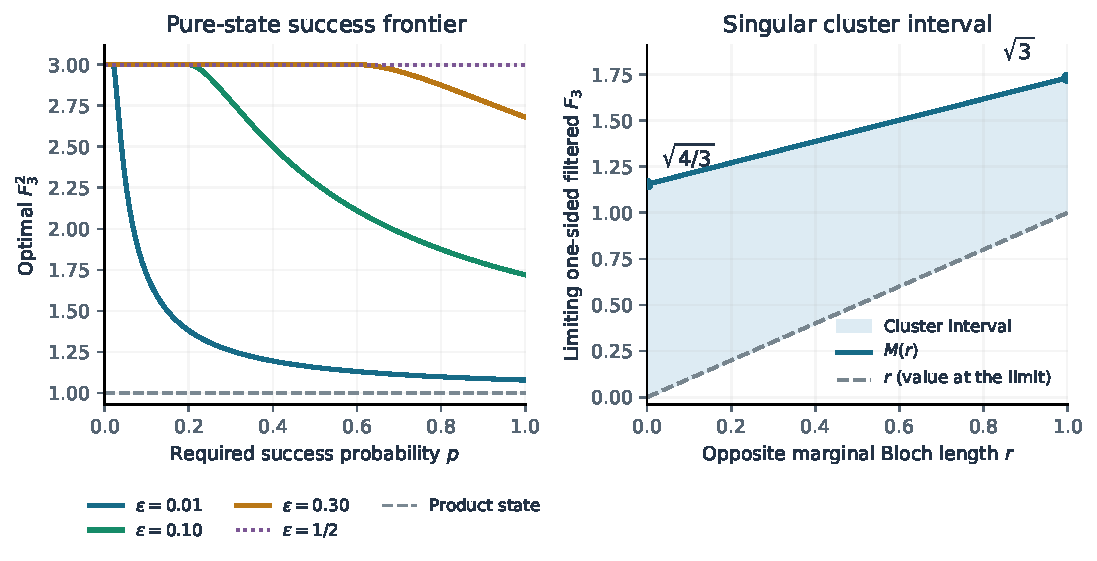
\includegraphics[width=\textwidth]{figures/operational_frontiers.pdf}
\caption{Exact analytical curves, without numerical filter optimization.
Left: the pure-state frontier in Theorem \ref{thm:purefrontier}; its Bell plateau
ends at $p=2\varepsilon$. Right: every value in the shaded interval is a cluster
value at the corresponding pure-marginal product state, by
Theorem \ref{thm:clusters}. A fixed positive rate restores continuity across
these singular limits. The figure is reproduced by \texttt{checks/make\_figures.py}.}
\end{figure}


\section{Research process and AI disclosure}\label{sec:disclosure}

This work is fully autonomous agentic research. Autonomous AI research
agents produced the results, the written proofs, the exact and numerical
checkers and the Lean development in an earlier session, starting from the
open question of Ducuara, Susa and Skrzypczyk \cite{ducuara}. The records
of that session describe internal audits carried out within the same
automated workflow; they are internal AI-assisted reviews, not peer review,
and they are not included. Opus~5.5 by Anthropic used with Claude Code
assessed the package for this release: it checked the source question and
the cited equations, read the proofs of Theorems~\ref{thm:main}
and~\ref{thm:violation} and of Proposition~\ref{prop:galois}, reran every
checker from a copy, wrote and ran the brute-force comparison, rebuilt the
Lean project module by module with a new whole-project axiom audit, checked
the formal statement against actual density matrices and filters, edited
the manuscript and integrated the package into the repository. The
mathematics of the extensions was not changed. Dev D. Goyal is responsible
for publication. The work has not been externally peer reviewed. The formal
scope is stated in Appendix~\ref{sec:formal}; the remaining results rest on
the written proofs and the checks of Appendix~\ref{app:checks}.

The Lean library in \texttt{lean/QuantumPrior} is adapted, with
attribution, from the author's earlier formalization of steering-ellipsoid
results, from which the companion package \cite{steeringbounds} was
released. It contains the fully-entangled-fraction bound
$f(\rho)\leq1-c/2$, which is Conjecture~2 of Milne, Jennings, Jevtic and
Rudolph \cite{milnemaxmixed}. The Omega Institute's public repository
records a claimed Lean proof of that conjecture committed on 8 October 2026
(issue \#14206), and a proof of their Conjecture~1, on the CHSH value at
fixed centre, committed on 14 October 2026 (issue \#16558). No priority is
claimed for either statement; neither is used in the main theorem here, and
neither record contains the one-sided filtered measures.

\appendix
\part*{Appendices}
\addcontentsline{toc}{part}{Appendices}

\section{Independent verification and reproducibility}\label{app:checks}

All programs are in the package directory \texttt{checks/}. The command
\begin{verbatim}
python3 checks/run_checks.py --independent
\end{verbatim}
replays them in a temporary copy with \texttt{python3 -I}.

\paragraph{Primary numerical implementation.}
\texttt{f3\_exact.py} evaluates the finite spectral prescription and
reconstructs valid Kraus operators. \texttt{verify.py} uses seed
$20261103$, generates $400$ random density matrices, $100$ of each rank
$1,2,3,4$, and checks both filtering directions ($800$ instances).
It checks the original fractional identity, canonicalization, ellipsoid
shape, reconstructed density matrices, the exact gap identity as a numerical
identity, and the spectral prescription, with explicit singular examples.
The maximum recovered-filter squared-value discrepancy was
$9.09\times10^{-13}$; the largest gap-identity residual was
$8.33\times10^{-16}$. The secondary nonsymmetric shape-spectrum check had
maximum discrepancy $3.47\times10^{-9}$, reflecting repeated-root
conditioning. These are floating-point checks and are not substituted for
the proofs.

\paragraph{Separate implementation.}
\texttt{independent\_check.py} was written separately. It whitens through
$2\times2$ marginal eigendecomposition and directly filters $4\times4$
density matrices, rather than reusing the primary Bloch implementation.
It checks $240$ independently generated rank-$1$--$4$ states plus named
cases ($514$ one-sided instances). The largest reconstruction discrepancy
was $3.26\times10^{-13}$. For $64$ instances it also compared against
multistart constrained optimization, with maximum absolute discrepancy
$1.70\times10^{-7}$ and no observed optimizer excess above the formula
larger than $1.78\times10^{-15}$. No failed checks were recorded.

\paragraph{Brute-force comparison.}
\texttt{independent\_bruteforce.py} was written for this release and shares
no code with the other programs. For $24$ random states of ranks $1$--$4$,
some mixed with the maximally mixed state, it maximizes $F_3$ of the
normalized Alice-filtered $4\times4$ state over the eight real parameters
of a complex $2\times2$ filter by multistart Nelder--Mead and compares the
result with a fresh implementation of Theorem~\ref{thm:main}. The search
never exceeded the formula by more than $10^{-8}$ and reached it within
$10^{-6}$ in every case. In the hard case the top eigenvalue of
$\mathscr M$ can be defective, and a floating-point eigenvalue routine
then returns a nearly real pair; the comparison therefore accepts
eigenvalues with imaginary part below $10^{-6}$ as real. A first version
with a tighter tolerance missed such a root in one case; this was an error
of the comparison program, which the exact evaluators avoid.

\paragraph{Exact arithmetic.}
\texttt{verify\_galois\_certificate.py} uses Python's standard library,
exact fractions and finite-field arithmetic. It reconstructs the sextic,
verifies modular products, squarefreeness, and irreducibility, and supplies
rational root/value enclosures. The finite checks support the explicitly
written Galois argument; the program is not a Lean proof of field theory.

\paragraph{Exact evaluation for rational states.}
\texttt{exact\_rational.py} accepts rational original Bloch data and checks
all fifteen nonempty principal minors of the resulting Hermitian density
matrix. It constructs the six invariant coefficients using rational arithmetic,
isolates the ordered real roots of the sextic, and uses an exact Sturm count
to choose the branch $\eta=\max(d,\nu)$. At a spectral pole, divisibility by
the minimal polynomial determines the first nonzero derivative in
Corollary~\ref{cor:sixinvariants}; quotient-field reduction then certifies
the returned value. No floating-point approximation chooses a branch or
accepts a value. \texttt{verify\_exact\_rational.py} passes $23$ exact cases,
covering both parties, all derivative orders $0,1,2,3$, the nonzero-gradient
hard case, flat optima, pure marginals, rational pure entangled states, and
the degree-six Galois example. It also checks exact invariance under a
rational orthogonal rotation and reconstructs determinant and adjugate
identities independently. \texttt{verify\_companion\_exact.py} checks the
companion determinant in exact integer arithmetic in dimensions $1$--$4$,
including singular shifts, and the six-invariant compression.

\paragraph{Operational and conditional-state checks.}
\texttt{extension\_checks.py} checks $48$ physical states at $144$
probability budgets, using $1008$ independent constrained-optimizer starts.
The maximum reconstructed squared-value error is $1.43\times10^{-13}$;
the maximum comparison discrepancy is $1.33\times10^{-9}$.
It also checks $96$ arbitrary affine optimal families, $72$ boundary-only
families against $80$ directions each, and $27$ pure-state frontier cases.
The reference solver for the rate reports numerical success in $69$ of
$96$ cases; all $96$ endpoint values nevertheless agree within
$6.14\times10^{-10}$. The JSON report preserves those statuses.
A scalar rate expression loses $2.87\times10^{-8}$ near a double root,
while direct Hermitian effect evaluation remains accurate to
$6.11\times10^{-15}$.
\texttt{conditional\_checks.py} tests $384$ projections from $48$ physical
states, the complex block identity, invariance under invertible filters,
seven exact equality families, and $21$ collapsing states. The largest
block-identity residual is $6.67\times10^{-16}$ and the largest
conditional-state invariance error is $2.65\times10^{-15}$. Five exact
symbolic identities also pass. These checks detect errors; the analytical
proofs are the source of the universal claims.

\section{Formal verification}\label{sec:formal}

\paragraph{The end-to-end theorem.}
The Lean declaration
\texttt{FilteredF3.\allowbreak equation10\_\allowbreak both\_\allowbreak closed\_\allowbreak forms} states, for every
\texttt{M : Milne.CMatrix} (a complex matrix indexed by pairs of qubit
indices) satisfying \texttt{Milne.Density M} (positive semidefinite with
trace one), that
\[
 \operatorname{IsLUB}(\mathcal V_A(\rho),\sqrt{V_A(\rho)})
 \quad\text{and}\quad
 \operatorname{IsLUB}(\mathcal V_B(\rho),\sqrt{V_B(\rho)}).
\]
Here $\mathcal V_A$ is the set of values $\sqrt{\sum_{i,j}T_{ij}^2}$, with
$T_{ij}=\operatorname{Re}\tr(\rho'\,\sigma_i\otimes\sigma_j)$, over the
states $\rho'=(K\otimes I)\rho(K\otimes I)^\dagger/p$ for complex
$2\times2$ matrices $K$ with $\det K\neq0$ and success trace $p>0$;
$\mathcal V_B$ is the same with $I\otimes K$. There are no rank
assumptions on the state or its marginals. The right side $V_B$ is
$\norm a^2$ when Bob's marginal is singular, and otherwise the spectral
value of the canonical quadratic of the whitened state, computed from
mathlib's orthonormal eigenbasis of a real symmetric $3\times3$ matrix and
the greatest real root of the explicit secular polynomial, whose existence
is proved; $V_A$ is $V_B$ of the swapped state. The definitions contain no
optimization over filters and no assumed optimizer or certificate.

\paragraph{What the formal chain proves.}
The development proves the filtering-to-quadratic identity for actual
matrices and the equality of the complete value sets, removes the canonical
assumption by whitening and Pauli reconstruction, proves the product
factorization at a pure filtered marginal, normalizes by the success
probability and exchanges the parties by an explicit matrix swap.
Invertibility of the filter is proved equivalent to the open Bloch ball, and
continuity and density show that the open-ball supremum equals the
closed-ball maximum. On the spectral side it proves the exact gap identity,
root and optimizer existence for every finite diagonal quadratic, the
transfer to arbitrary real symmetric matrices, a singular-safe
block-determinant identity for the companion matrix, all maximizing
coordinates and kernel freedoms, the extremizing filters and the
characterization of attainment by invertible filters, and the rational
violating-branch criterion in canonical coordinates. Additional modules
prove scalar radius, convexity, gap-stability and parabola lemmas used by the
extensions.

\paragraph{Not formalized.}
The rational Bloch-coordinate expressions for $(c,Q)$ in
Theorem~\ref{thm:main}, the direct fractional numerator, the six-invariant
rule of Corollary~\ref{cor:sixinvariants}, the separability corollary, the
Galois obstruction, the two-ball success frontier and its candidate
enumeration, the highest-success branch rule, continuity and the
discontinuity locus, the pure-state frontier, the physical
conditional-purity bound and its equality family, and the cluster interval
are written proofs with the checks described above; for the last of these
only a scalar lemma is formalized. The Lean functional is the Frobenius
expression of Equation~(3) of \cite{ducuara}; its derivation from the
optimization over measurement settings is cited, not formalized. The value
sets use invertible matrices up to scale; the rescaling to a contractive
physical filter is in the written proof.

\paragraph{Build and audit.}
The project in \texttt{lean/} pins Lean~4.19.0 and mathlib revision
\texttt{c44e0c8e\allowbreak e63ca166\allowbreak 450922a3\allowbreak 73c7409c\allowbreak 5d26b00b}. Its 43 modules keep the
names of the original development; 22 of them, in \texttt{QuantumPrior},
are the attributed library described in Section~\ref{sec:disclosure}. For this release
the project was built module by module from source with
\texttt{lake build}, and the module \texttt{AxiomAudit} enumerates every
declaration whose defining module is one of the 41 modules that define
declarations, including private and compiler-generated ones, and checks its
transitive axioms with Lean's own collector. The audit covers 850
declarations, including all 490 named in the sources. The 604 declarations
other than Lean~4.19 code-generation auxiliaries, among them the 503
theorems, depend only on \texttt{propext}, \texttt{Classical.choice} and
\texttt{Quot.sound}; the 246 auxiliaries depend in addition only on other
auxiliaries and, for 11 of them, on the code generator's placeholder
\texttt{lcProof}. The fresh build compiled all 43 modules and the audit
from source against the pinned mathlib cache. The sources contain no
\texttt{sorry}, \texttt{admit}, \texttt{axiom} declaration,
\texttt{native\_decide} or \texttt{ofReduceBool}.


\begin{thebibliography}{99}
\bibitem{ducuara}
A. F. Ducuara, C. E. Susa, and P. Skrzypczyk,
\emph{Locally inaccessible hidden quantum correlations},
Physical Review A \textbf{110}, 022435 (2024).
\href{https://arxiv.org/abs/2406.03945}{arXiv:2406.03945};
\href{https://doi.org/10.1103/PhysRevA.110.022435}{doi:10.1103/PhysRevA.110.022435}.
Equation numbers refer to arXiv version~1.

\bibitem{costa}
A. C. S. Costa and R. M. Angelo,
\emph{Quantification of Einstein--Podolsky--Rosen steering for two-qubit states},
Physical Review A \textbf{93}, 020103(R) (2016).
\href{https://doi.org/10.1103/PhysRevA.93.020103}{doi:10.1103/PhysRevA.93.020103}.

\bibitem{cjwr}
E. G. Cavalcanti, S. J. Jones, H. M. Wiseman, and M. D. Reid,
\emph{Experimental criteria for steering and the Einstein--Podolsky--Rosen paradox},
Physical Review A \textbf{80}, 032112 (2009).
\href{https://doi.org/10.1103/PhysRevA.80.032112}{doi:10.1103/PhysRevA.80.032112}.

\bibitem{jevtic}
S. Jevtic, M. Pusey, D. Jennings, and T. Rudolph,
\emph{Quantum steering ellipsoids},
Physical Review Letters \textbf{113}, 020402 (2014).
\href{https://doi.org/10.1103/PhysRevLett.113.020402}{doi:10.1103/PhysRevLett.113.020402}.

\bibitem{milne}
A. Milne, S. Jevtic, D. Jennings, H. Wiseman, and T. Rudolph,
\emph{Quantum steering ellipsoids, extremal physical states and monogamy},
New Journal of Physics \textbf{16}, 083017 (2014).
\href{https://doi.org/10.1088/1367-2630/16/8/083017}{doi:10.1088/1367-2630/16/8/083017}.

\bibitem{milnemaxmixed}
A. Milne, D. Jennings, S. Jevtic, and T. Rudolph,
\emph{Quantum correlations of two-qubit states with one maximally mixed marginal},
Physical Review A \textbf{90}, 024302 (2014).
\href{https://arxiv.org/abs/1404.3951}{arXiv:1404.3951}.

\bibitem{steeringbounds}
D. D. Goyal,
\emph{Exact three-setting correlation bounds at fixed steering centre},
preprint (2026),
\url{https://github.com/dvgyl/math-and-theory/tree/main/papers/physics/steering-bounds}.

\bibitem{adachi}
S. Adachi, S. Iwata, Y. Nakatsukasa, and A. Takeda,
\emph{Solving the trust-region subproblem by a generalized eigenvalue problem},
SIAM Journal on Optimization \textbf{27}(1), 269--291 (2017).
\href{https://doi.org/10.1137/16M1058200}{doi:10.1137/16M1058200}.
This paper credits the earlier spectral reduction of Gander, Golub, and
von Matt (1989). The general spectral trust-region method is not claimed
as new here.
\bibitem{twoballs}
S. Ansary Karbasy and M. Salahi,
\emph{Quadratic optimization with two ball constraints},
Numerical Algebra, Control and Optimization \textbf{10}(2), 165--175 (2020).
\href{https://doi.org/10.3934/naco.2019046}{doi:10.3934/naco.2019046}.

\bibitem{rontsis}
N. Rontsis, P. J. Goulart, and Y. Nakatsukasa,
\emph{An active-set algorithm for norm constrained quadratic problems},
Mathematical Programming \textbf{193}, 447--483 (2022).
\href{https://doi.org/10.1007/s10107-021-01617-2}{doi:10.1007/s10107-021-01617-2}.

\bibitem{vidal}
G. Vidal, \emph{Entanglement of pure states for a single copy},
Physical Review Letters \textbf{83}, 1046--1049 (1999).
\href{https://arxiv.org/abs/quant-ph/9902033}{arXiv:quant-ph/9902033};
\href{https://doi.org/10.1103/PhysRevLett.83.1046}{doi:10.1103/PhysRevLett.83.1046}.

\bibitem{ku}
H.-Y. Ku et al., \emph{Complete classification of steerability under local
filters and its relation with measurement incompatibility},
Nature Communications \textbf{13}, 4973 (2022).
\href{https://doi.org/10.1038/s41467-022-32466-y}{doi:10.1038/s41467-022-32466-y}.
Filtering equivalence and success-probability questions are studied for
steering assemblages, a different resource from the invariant optimized here.

\bibitem{probabilityprior}
A. F. Ducuara, C. E. Susa, and J. H. Reina,
\emph{Emergence of maximal hidden quantum correlations and its trade-off
with the filtering probability in dissipative two-qubit systems},
Physica A \textbf{594}, 127035 (2022).
\href{https://doi.org/10.1016/j.physa.2022.127035}{doi:10.1016/j.physa.2022.127035}.

\bibitem{horodecki}
M. Horodecki, P. Horodecki, and R. Horodecki,
\emph{Separability of mixed states: necessary and sufficient conditions},
Physics Letters A \textbf{223}, 1--8 (1996).
\href{https://arxiv.org/abs/quant-ph/9605038}{arXiv:quant-ph/9605038};
\href{https://doi.org/10.1016/S0375-9601(96)00706-2}{doi:10.1016/S0375-9601(96)00706-2}.

\end{thebibliography}
\end{document}
